% Nejprve uvedeme tridu dokumentu s volbami
\documentclass[czech,public,dept460,male,cpdeclaration]{diploma}
% Dalsi doplnujici baliky maker
\usepackage{subfig}		% makra pro "podobrazky" a "podtabulky"
\usepackage{tikz}		% makra pro kresleni
\usepackage{fancyvrb}

% Zadame pozadovane vstupy pro generovani titulnich stran.
\ThesisAuthor{Adam Lasák}

\CzechThesisTitle{Simulace davu}

\EnglishThesisTitle{Crowd Simulation}

\SubmissionDate{26. dubna 2018}

% Pokud nechceme nikomu dekovat makro zapoznamkujeme.
\Thanks{Tímto bych rád poděkoval svému vedoucímu, Ing. Martinu Němcovi, Ph.D., za poskytnuté \newline
odborné rady, za neocenitelné zkušenosti a za všechen čas, jenž mi takto věnoval.}

% Zadame cestu a jmeno souboru ci nekolika souboru s digitalizovanou podobou zadani prace.
% Pokud toto makro zapoznamkujeme sazi se stranka s upozornenim.
\ThesisAssignmentImagePath{Figures/Assignment}

% Zadame soubor s digitalizovanou podobou prohlaseni autora zaverecne prace.
% Pokud toto makro zapoznamkujeme sazi se cisty text prohlaseni.
%\AuthorDeclarationImageFile{Figures/AuthorDeclaration.jpg}

%\ThesisAccessRestriction{Zde vložte text dohodnutého omezení přístupu k Vaší práci, chránící například firemní know-how. Zde vložte text dohodnutého omezení přístupu k Vaší práce, chránící například firemní know-how. A zavazujete se, že:
%\begin{enumerate}
%\item podle \textsection{} 5 o práci nikomu neřeknete,
%\item po obhajobě na ni zapomenete a
%\item budete popírat její existenci.
%\end{enumerate}
%A ještě jeden důležitý odstavec. A ještě jeden důležitý odstavec.
%A ještě jeden důležitý odstavec. A ještě jeden důležitý odstavec.
%A ještě jeden důležitý odstavec. A ještě jeden důležitý odstavec.
%Konec textu dohodnutého omezení přístupu k Vaší práci.}

% Zadame soubor s digitalizovanou podobou souhlasu spolupracujici prav. nebo fyz. osoby.
% Pokud toto makro zapoznamkujeme sazi se cisty text souhlasu.
%\CooperatingPersonsDeclarationImageFile{Figures/CoopPersonDeclaration.jpg}

\CzechAbstract{Spousta věcí v přírodě je stejně působivých jako zvířata, která se mohou organizovat do větších a logicky orientovaných seskupení.
Tím že dokážeme simulovat toto chování, můžeme vytvořit reálnou podobu davu. Reálné využití pak najdeme v konkrétních oborech lidské činnosti: návrhy veřejných budov, filmové projekty či programování PC her.
Tato práce se zaměřuje na popis boidova algoritmu, který je dnes nejpoužívanější co se simulace davu týče.}

\CzechKeywords{Boidův algoritmus, dav, hejno, koheze, separace, zarovnání, agent}

\EnglishAbstract{Many things in nature are impressive like animals which can be organized into larger and logical oriented grouping.
In that case when we can simulate this behavior than we can create real form of the crowd. Real use can be found in things like: creating public buildings, movie projects or developing games.
This thesis focuses on the description of boid's algorithm which is the most used crowd simulation principle today. }

\EnglishKeywords{Boid's algorithm, crowd, flock, cohesion, separation, alignment, agent}

\AddAcronym{ACM}{Association for Computing Machinery - vědecky-vzdělávací instituce pro výpočetní technologie}
\AddAcronym{AI}{Artificial Intelligence - umělá inteligence}
\AddAcronym{FPS}{Frames per seconds - počet snímku za jednu sekundu}
\AddAcronym{GLEW}{OpenGL Extension Wrangler Library - poskytuje realtime prostředky pro danou platformu}
\AddAcronym{GLFW}{Graphics Library Framework - Multiplatformní technologie rozšiřující OpenGL o vytváření aplikačních oken}
\AddAcronym{GLM}{OpenGL Mathematics - poskytuje širokou škálu matematických operací pro OpenGL}
\AddAcronym{GPU}{Graphics processing unit – grafická karta, má svůj procesor i~výpočetní paměť}
\AddAcronym{IDE}{Integrated Development Environment - program usnadňující práci programátorům}
\AddAcronym{Particle System}{Definuje shluky malých částic s podobným chováním a vlastnostm}
\AddAcronym{RAM}{Random Access Memory – operační paměť počítače}
\AddAcronym{Realtime}{Vykreslování v reálném čase – snaha vykreslovat co nejrychleji}
\AddAcronym{SIGGRAPH}{Special Interest Group on Computer GRAPHics and Interactive Techniques - výroční konference v počítačové grafice}

% Zacatek dokumentu
\begin{document}

% Nechame vysazet titulni strany.
\MakeTitlePages

% Pokud mame v zaverecne praci vypisy kodu, jinak odstranit.
\lstlistoflistings

\section{Úvod}
Simulační algoritmy se používají v širokém spektru odvětví od vědy, her, výpočetních úkonů až po kinematografii či stavbu budov \cite{linkToBuildingSimulation}. Herní využití mívá velmi reálně implementována armáda \cite{linkToArmySimulation}, která tímto způsobem zaškoluje vojáky ve virtuálním simulačním boji jak v taktice, tak způsobu nejefektivnějšího využití dostupných zbraní. 

Pokud vezmeme v potaz stavbu či projektování budov, nabízí se další subspektra  druhů simulačních programů. Například projektant potřebuje nasimulovat jak velkou zátěž udrží hlavní nosníky, testování a simulování různých druhů materiálů či jak velké budou úniky tepla na základě pohybů osob v budově.

Avšak po této základní konstrukční stránce, se musí také navrhnout optimální velikost budovy a kolik bude schopna pojmout lidí v jednom okamžiku. Kde bude vést úniková cesta v případě požáru a kolik času zabere evakuovaným lidem \textit{(davu)}, než se z budovy dostane do bezpečí. A~zrovna~co se bezpečnosti týče, mají simulační algoritmy nejširší využítí. V jistém slova smyslu by se dalo říci, že byly vytvořeny primárně pro tento účel \cite{link1}.

Při těchto simulacích se tak navrhují nejlepší varianty šířky chodeb, dostupnosti k únikovým východům, přístupu k požárnímu schodišti nebo vyladění ukazatelů směru
úniku.

Pokročilejší algoritmy také reagují na různé překážky, jak horizontální tak vertikální. Dokáží simulovat dav, který jde z jednoho patra do druhého různými typy cest a střetává se tak s jinými davy. Cílem projektanta je pak vybrat vhodné únikové cesty z budovy a zpracovat nejoptimálnější únikový plán.

V této práci se seznámíme se základy simulování davu a hejna. Popíšeme nejpoužívanější algoritmus \cite{link2} pro tento druh simulace a realizaci výsledné aplikace.

\section{Simulace}
Pojem simulace lze vydefinovat: \textit{"Počítačová simulace je napodobení skutečnosti pomocí numerického výpočtu, nezbytná součást modelování fyzikálních procesů. Dokáže předpovědět jak kvantitativní, tak kvalitativní výsledky pokusů při různých počátečních podmínkách. Umožňuje omezit výběr jevů, které celý pokus ovlivňují nejvíce a tím vysvětlit příčiny a podstatu procesů."} (Citace \cite{linkToSimulation})

V našem případě se jedná o napodobení davu, kdy pomocí algoritmu dokážeme předem modifikovat nadcházející krok a tím i změnit výsledné chování celého davu. Na základě vstupních dat nebo kombinací pravidel můžeme chování měnit a tím simulovat dav při různých situacích, jako je evakuace z budovy nebo běžné chození po prostorách nákupního střediska.

\subsection{Simulace davu}
Existují v zásadě dvě možnosti, jak simulovat dav lidí. Částicová simulace a simulace založená na umělé inteligenci. \cite{linkToBachelor1}

\subsection{Částicová simulace}
První zmíněná simulace je založena na principu přiřazení hmotného bodu každému chodci ve scéně, jehož pohyb je odvíjen působením nejrůznějších sil. Hlavní výhoda spočívá v nasimulování velkého množství lidí z důvodu nenáročnosti výpočtů na výpočetní výkon, ale výsledná vizualizace není příliš reálná. Příklady pro využití jsou typy založené na: magnetických silách, buněčném modelu a sociálních silách. \cite{linkToBachelor1}

\subsection{Simulace na bázi AI (Artificial Intelligence)}\label{sec:simulace-na-bazi-ai-artificial-intelligence}
Druhý zmíněný typ je založen na bázi Agentů. Ti už nejsou reprezentováni jen obyčejnými silami \textit{(i přesto že se jedná o diametrálně odlišný typ simulace davu, určité fyzikální vlastostni agenti stále musí mít)} ale také přidanými vlastnostmi, kterými předchozí typ tolik nedisponoval. Mají hlavně přidané senzory, díky nímž dokáží vyhodnocovat danou situaci v reálném čase a následně se rozhodovat k dalšímu nejvýhodnějšímu kroku. Pokud do scény vložíme dva a více agentů kteří budou na sebe reagovat, můžeme říci, že každý z nich má v jisté míře svůj mozek. Ať už jednodušší \textit{(rozhodování dalšího kroku mezi zdmi)} nebo složitější \textit{(např.: agent může v danou chvíli reagovat, zda-li má jít rychleji či pomaleji aby nezpůsobil kolizi s jiným agentem či agenty)}.

Tento typ simulace hojně využívá herní průmysl, kdy v nějaké scéně - herní mapě, jsou nasazeny desítky agentů, kteří se ve své podstatě starají sami o sebe a přímo či nepřímo komunikují s uživatelem. Obecně však platí, že ve hrách je tato implementace mnohonásobně složitější než částicová simulace kvůli mnoha vlastnostem agentů. Konkrétními případy může být třeba hra Crysis \textit{(leden 2007 - stáda jelenů)} a FarCry \textit{(2004 - hejna tropických papoušků \cite{linkToCrytek})}.

Je třeba také zminit kinematografický průmysl, který simuluje davy lidí. Tím pádem animátorům odpadne kus práce, kdy by museli každého agenta animovat zvlášť.

Jelikož byl v této práci využit tento typ simulace, tak v dalších kapitolách budeme každý bod ve scéně nazývat \textbf{``agentem''}.

\begin{figure}\centering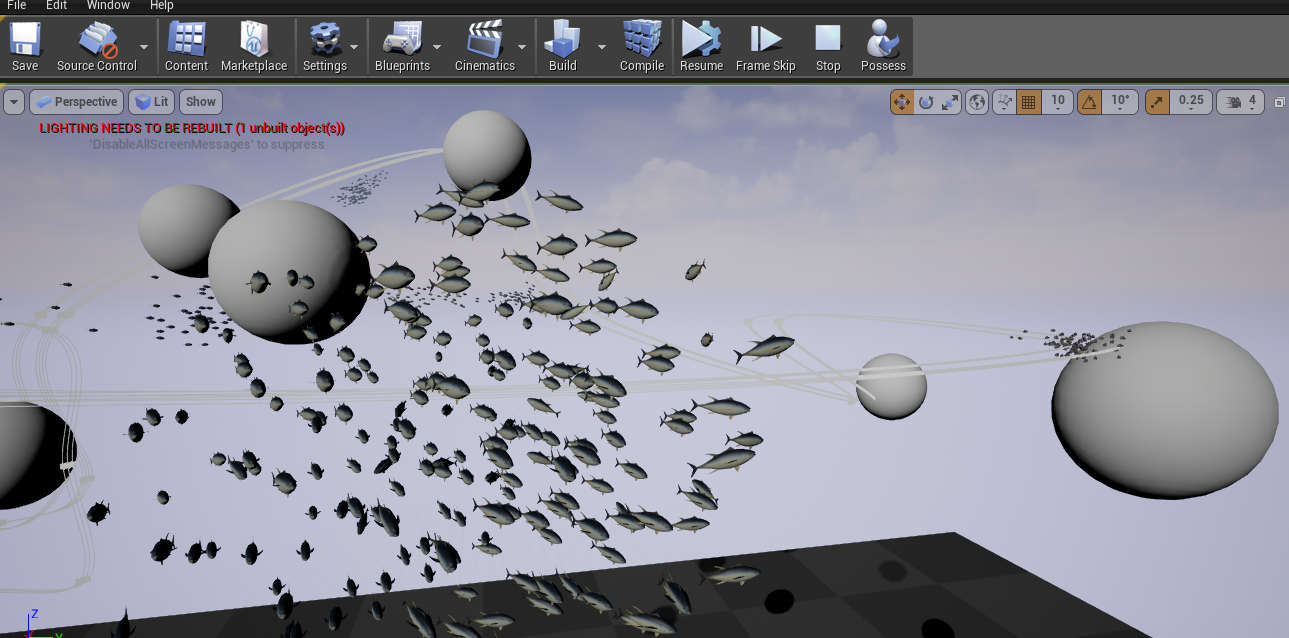
\includegraphics[width=0.8\textwidth]{Figures/flock_fish.png}
	\caption{
		Ukázka simulace hejna ryb v Unreal Enginu 4 (Zdroj: \cite{linkToUnrealEngineFish})
	}
\end{figure}

\subsection{Boidův algoritmus}\label{sec:boiduv-algoritmus}

Nejčastějším typem simulace založené na umělé inteligenci je Boidův algoritmus  vytvořený v roce 1986 Craigem Reynoldem a oficiálně představený roku 1987 na konferenci ACM SIGGRAPH \cite{linkToACM, linkToSIGGRAPH}.

Název Boidův algoritmus je odvozen od \textbf{``boidů''} \textit{(zkratka z anglického bird-oid object)} což referuje na simlaci hejna ptáků. Jak již bylo zmíněno výše, simulace založená na
umělé inteligenci obsahuje základní prvky částicové simulace, ale má také něco navíc. Výjma senzorů mají také přehled o celkové geometrii celé scény. Tzn. že každý agent \textit{(boid)} má přehled o všech agentech v celé scéně. Pokud bychom tedy maximalizovali důležitá tři pravidla tohoto principu popsané níže, znamená to, že každý iteruje s každým.

Mezi částicové prvky Boidova algoritmu lze použit například tření, zrychlení nebo okamžitou rychlost. Reálně lze tření ještě rozdělit na tření válcove, tření způsobené protivětrem nebo pokud bychom určili jako objekt auto, můžeme použít další fyzikální vlastnosti jako točivý moment případně brzdná dráha.

Existuje však celá řada vylepšení, která se dají s tímto algoritmem provést, například simulace chování dopravy. Ta funguje jako tzv. chování založeného na řízení \textit{(Steering behaviors)} \cite{linkToSteeringBehaviors}. 

V této práci byla tato vylepšení použita, čímž lze chování davu více přiblížit realitě. Přidané fyzikální veličiny jsou již zmíněné: tření, zrychlení a okamžitá rychlost.

\newpage
Následuje popis Boidova algoritmu, který obsahuje tři základní vlastnosti:

\begin{enumerate}
	\item Separace \textit{(Separation)}
	\item Zarovnání \textit{(Alignment)}
	\item Koheze \textit{(Cohesion)}
\end{enumerate}

\subsection{Separace}\label{sec:separace}
Separace slouží k tomu, aby se dva a více agentů nepřiblížili příliš blízko sebe a tím vyvolali kolizi mezi sebou. Je to první a nejzákladnější vlastnost Boidova algoritmu bez které by nebylo možné vytvořit kompletní simulaci. 

Oddělení od ostatních agentů funguje na principu základních operací s vektory \textit{(2D nebo 3D)} a vytvoření pomyslného kruhu kolem každého agenta, který jej upozorní zda-li není příliš blízko jiného agenta. 

Následující kroky provedou separaci agentů: 

\begin{enumerate}
	\item Odečtení vektoru agenta od vektoru aktuálně kontrolovaného agenta:
			\[ \scalebox{1.2}{$v_{sub} = v_{current} - v_{actual}$} \]
			
			kde \( \scalebox{1.2}{$v_{sub}$} \) je výsledný vektor, \( \scalebox{1.2}{$v_{currrent}$} \) je vektor agenta, který je právě v iteraci a \( \scalebox{1.2}{$v_{actual}$} \) je vektor aktuálně kontrolovaného agenta.

	\item Normalizování výsledného vektoru z předhozího kroku:
	
			\[ \scalebox{1.2}{$v_{norm} = \sqrt{vx_{sub}^2 + vy_{sub}^2 + vz_{sub}^2}$} \]
			
			kde \( \scalebox{1.2}{$v_{norm}$} \) je výsledný normalizovaný vektor \( \scalebox{1.2}{$v_{sub}$} \).
	\item Vydělení výsledku kroku č. 2 vzdáleností těchto dvou agentů. Výsledek se přičítá k výslednému vektoru \( \scalebox{1.2}{$v_{sum}$} \). Matematický zápis pak vypadá následovně:
			%\[ \scalebox{1.2}{$d_{x} = vx_{current} - vx_{actual}$} \]
			%\[ \scalebox{1.2}{$d_{y} = vy_{current} - vy_{actual}$} \]
			%\[ \scalebox{1.2}{$d_{z} = vz_{current} - vz_{actual}$} \]
			\[ \scalebox{1.2}{$v_{distance} = \sqrt{d_x^2 + d_y^2 + d_z^2}$} \]
			\[ \scalebox{1.2}{$v_{divide} = \frac{v_{norm}}{v_{distance}}$} \]
			\[ \scalebox{1.2}{$v_{sum} = v_{sum} + v_{divide}$} \]
						
			kde \( \scalebox{1.2}{$d_{x}$} \), \( \scalebox{1.2}{$d_{y}$} \) a \( \scalebox{1.2}{$d_{z}$} \) jsou rozdíly daných souřadnic mezi agentem v iteraci a aktuálně kontrolovaným agentem, \( \scalebox{1.2}{$v_{distance}$} \) je výsledný vektor vzdálenosti mezi těmito dvěma agenty a~\( \scalebox{1.2}{$v_{divide}$} \) je výsledek vydělení vektorů.
			
	\item Pokud je v okolí agenta více agentů se kterými koliduje, pak se na konci výsledný vektor vydělí počtem těchto agentů (viz obrázek č. \ref{fig:separationImg}).
\end{enumerate}

\begin{figure}[H]\centering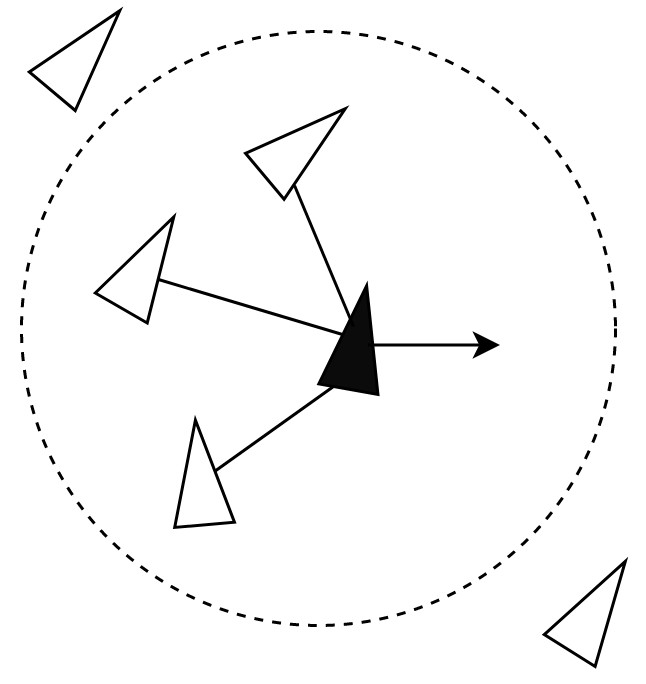
\includegraphics[width=0.4\textwidth]{Figures/separation2.jpg}\label{fig:separationImg}
	\caption{Separace - vyhýbání se ostatním agentům (Zdroj: vlastní)}\label{fig:separationImg}
\end{figure}

\begin{lstlisting}[language=c++,label=src:Separation pseudocode,caption=Pseudokód pro separaci (Zdroj: vlastní)]
function Separation(boid paramBoid)
{
	Vector result
	int count
	
	for (b in allBoids) {
		if (b != paramBoid){
			distance = distanceBetween(b, paramBoid)
			if (distance < SEPARATION_DIAMETER){
				sub = substractVectors(b, paramBoid) // b - paramBoid
				normalize(sub)
				divideScalar(sub, distance) // sub / distance
				result = result + sub
				count = count + 1
			}
		}
	}
	
	return divideScalar(result, count) // result / count
}
\end{lstlisting}

\subsection{Zarovnání}\label{sec:zarovnani}
Dalším důležitým pravidlem pro fungování Boidova algoritmu je zarovnání. Spolu se separací bez koheze má dav již základní podobu chování. 

Zarovnání má za úkol soudržnost. Všem agentům ve scéně poskytuje schopnost sladit se, jak je zobrazeno na obrázku č. \ref{fig:zarovnani}. 

Princip fungování je obdobný jako u separace, pokud se v blízkosti okruhu od daného agenta objeví jiný agent případně agenti, zprůměruje se jejich rychlost a směr a na základě těchto údajů modifikujeme údaje konkrétního agenta a tím zajístíme soudržnost všech dohromady. 

Pokud bychom chtěli aplikovat zarovnání a konkretizovat průběh, musíme se držet těchto kroků:

\begin{enumerate}
	\item V cyklu, který prochází všechny agenty ve scéně se testuje vzdálenost konkrétního agenta od jiného, který je momentálně v dané iteraci cyklu pod určitým indexem. Pokud je tato vzdálenost menší než průměr kruhu, přičtou se souřadnice vektoru daného agenta k lokálnímu sumárnímu vektoru \( \scalebox{1.2}{$v_{sum}$} \). Matematický zápis vypadá následovně:
	
		\[ \scalebox{1.2}{$v_{distance} = \sqrt{d_x^2 + d_y^2 + d_z^2}$} \]
		\[ \scalebox{1.2}{$v_{sum} = v_{sum} + v_{divide}$} \]
		
		kde \( \scalebox{1.2}{$d_{x}$} \), \( \scalebox{1.2}{$d_{y}$} \) a \( \scalebox{1.2}{$d_{z}$} \) jsou rozdíly daných souřadnic mezi agentem v iteraci a aktuálně kontrolovaným agentem, \( \scalebox{1.2}{$v_{distance}$} \) je výsledný vektor vzdálenosti mezi těmito dvěma agenty.
		
	\item Jestliže se podmínka nesplnila a tudíž sumární vektor \( \scalebox{1.2}{$v_{sum}$} \) je roven nule, pak se pravidlo zarovnání ukončuje. Pokud se alespoň jednou podmínka v kroku č. 1 provedla, tak následují kroky:
	
	\begin{itemize}
		\item sumární vektor \( \scalebox{1.2}{$v_{sum}$} \) se vydělí skalární hodnotou rovné počtu splněných podmínek \\v kroku č. 1:
		
		\[ \scalebox{1.2}{$v_{sum} = \frac{v_{sum}}{c}$} \]
		
		kde \( \scalebox{1.2}{$c$} \) je počet splněných podmínek. 
		
		\item normalizování sumárního vektoru \( \scalebox{1.2}{$v_{sum}$} \):
		
		\[ \scalebox{1.2}{$v_{sum} = \sqrt{vx_{sum}^2 + vy_{sum}^2 + vz_{sum}^2}$} \]
		
		\item vypočtení výsledného vektoru dle kterého se upraví směr daného agenta vzorcem: 
		\[ \scalebox{1.2}{$v_{res} = v_{sum} - v_{velocity}$} \]
		kde \( \scalebox{1.2}{$v_{sum}$} \) je sumární vektor a \( \scalebox{1.2}{$v_{velocity}$} \) je rychlost aktuálně kontrolovaného agenta.
	\end{itemize}
	
\end{enumerate}

\begin{figure}[H]\centering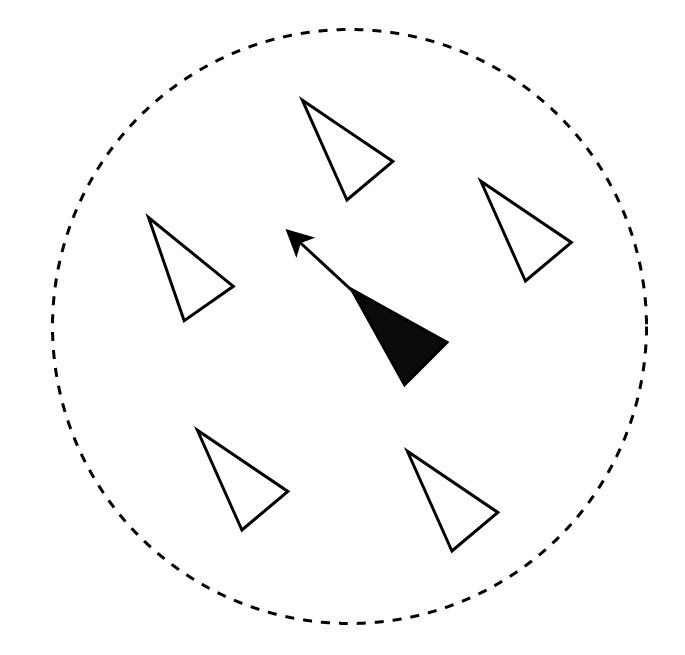
\includegraphics[width=0.4\textwidth]{Figures/alignment2.jpg}
	\caption{Zarovnání - určení směru agenta vůči průměrnému směru ostatních (Zdroj: vlastní)} \label{fig:zarovnani}
\end{figure}

\begin{lstlisting}[language=C++,label=src:Alignment pseudocode,caption=Pseudokód pro zarovnání (Zdroj: vlastní)]
function Alignment(boid paramBoid) {
	Vector sum
	int count
	
	for (b in allBoids) {
		if (b != paramBoid){
			distance = distanceBetween(b, paramBoid)
			if (distance < ALIGNMENT_DIAMETER){
				sum = sum + b.velocity
				count = count + 1
			}
		}
	}
	
	if (count > 0){
		divideScalar(sum, count) // sum / count
		normalize(sum)
		return substractVectors(sum, velocity) // sum - velocity
	} else {
		return sum
	}
}
\end{lstlisting}

\subsection{Koheze}\label{sec:koheze}
Při simulaci pomocí boidových třech pravidlech je koheze\footnote{Koheze je fyzikální síla držící pohromadě atomy či molekuly téže látky či tělesa (zejména
	kapalného a pevného tělesa), pozn. upraveno \cite{linkToCohesion}} tím nejméně důležitým pravidlem. Pokud bychom aplikovali pouze dvě předchozí pravidla a sice separaci a zarovnání, pak by výsledek už vykazoval známky chování davu.

Funguje na principu spojení okolních agentů \textit{(a následně vytvoření skupiny)}, kteří zasahují do dalšího pomyslného kruhu. Aby toto pravidlo fungovalo správně a nekolidovalo s podmínkami separace pak musí platit \(constCoh > constSep\), kde \(constSep\) je maximální průměr kružnice ve které se při překročení tohoto průměru řeší podmínky separace a \(constCoh\) je maximální průměr kružnice u koheze. Pokud by podmínka byla opačná, koheze se provede špatně nebo vůbec. Průměry kružnic koheze a zarovnání však na sebe vliv nemají.

Ve výsledné fázi se tedy musí určit průměrná lokace mezi všemi agenty kteří spadají do okruhu daného \textit{(aktuálně kontrolovaného)} agenta. Ve chvíli kdy se tyto souřadnice zjistí, agent na ně začne směřovat.

Následují dvě základní operace které provedou změnu směru daného agenta k průměrné lokaci ostatních agentů, kteří jsou v jeho okruhu.

\begin{enumerate}
	\item Hlavní cyklus který prochází všechny agenty ve scéně a kontroluje vzdálenosti ostatních agentů vůči konkrétnímu agentovi. Pokud libovolný agent spadá do okruhu nějakého konkrétního, opět se přičítá k sumárnímu vektoru \( \scalebox{1.2}{$v_{sum}$} \) avšak ne rychlost, ale lokace blízkého agenta.
	\item Následně se provede tentýž krok jako u zarovnání, čili sumární vektor \( \scalebox{1.2}{$v_{sum}$} \) se vydělí skalárem počtu splněných podmínek v kroku č. 1
	
\end{enumerate}

\begin{figure}[H]\centering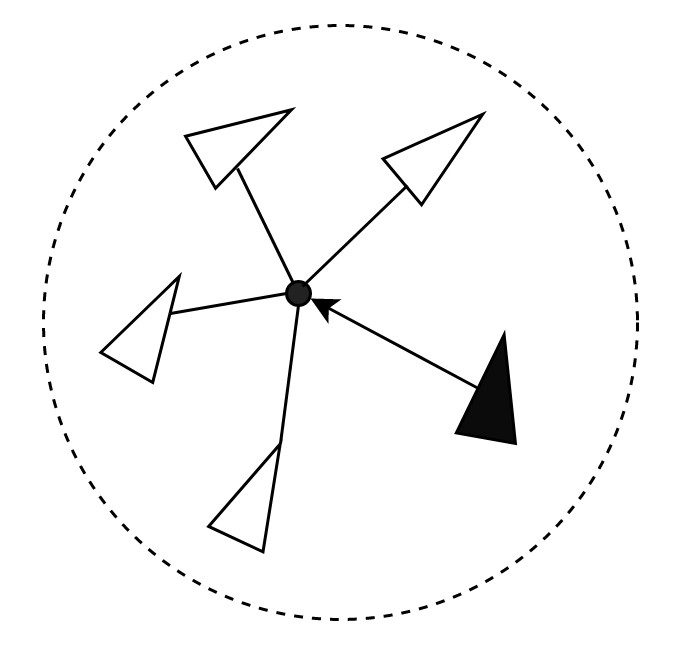
\includegraphics[width=0.4\textwidth]{Figures/cohesion2.jpg}
	\caption{Koheze - určení směru k průměrné lokaci okolních agentů (Zdroj: vlastní)}
\end{figure}

Kód v následujícím pseudokódu je obdobný jako kód zarovnání vyjma řádku s normalizováním sumárního vektoru, avšak v implementační části je tento kód složitější v řádku vracení výsledné hodnoty, kdy se ještě řeší fyzikální vlastnosti.

\begin{lstlisting}[language=c++,label=src:Cohesion pseudocode,caption=Pseudokód pro kohezi (Zdroj: vlastní)]
function Cohesion(boid paramBoid)
{	
	Vector sum
	int count
	
	for (b in allBoids) {
		if (b != paramBoid){
			distance = distanceBetween(b, paramBoid)
			if (distance < COHESION_DIAMETER){
				sum = sum + b.location
				count = count + 1
			}
		}
	}
	
	if (count > 0){
		divideScalar(sum, count) // sum / count
		return physicalProperty(substractVectors(sum, velocity))
	} else {
		return sum
	}
}
\end{lstlisting}

\subsection{Aplikování tří pravidel}\label{sec:aplikovani-tri-pravidel}
Ke kompletní simulaci dojde ve chvíli spojením třech výše zmíněných pravidel. Technicky vzato se jedná o sečtení všech třech výsledných vektorů z každé ze tří metod a rychlosti daného agenta který je aktuálně v iteraci. Nejdříve se sčítají rychlosti a poté se z této sumy spočítá výsledná pozice (Výpis pseudokódu č. 4).

Avšak pravidel je možné použít více, jak je popsáno v publikaci od Craiga Reynolda, Steering Behaviors For Autonomous Characters \cite{linkToSteeringBehaviors}. Tudíž nemusí být nutně tři fixní pravidla, ale můžeme k sčítání výsledných vektorů jednotlivých pravidel připsat i pravidla jiná. Kombinacemi těchto pravidel lze dosáhnout různého výsledného chování agentů.

Následující pseudokód ukazuje, jak lze tato pravidla aplikovat.

\begin{lstlisting}[language=c++,label=src:Flocking pseudocode,caption=Pseudokód pro aplikování třech pravidel (Zdroj: vlastní)]
function AllBoidsToNewPosition()
{
	Vector v1, v2, v3
	Boid b
	
	for (b in allBoids) {
		v1 = Separation(b)
		v2 = Alignment(b)
		v3 = Cohesion(b)
		// v4 = anotherRule(b)
		
		b.velocity = b.velocity + v1 + v2 + v3
		b.position = b.position + b.velocity
	}

}
\end{lstlisting}

Tento algoritmus se ještě aplikuje do tzv. Flocking algoritmu, který všechny agenty ve scéně vytváří a koordinuje jejich průběh s vizualizací.

\newpage
\section{Praktická část}
Následující sekce se zabývá použitými technologiemi a celkové implementaci aplikace, v niž byla použita metoda simulace na bázi umělé inteligence \textit{(Artificial Intelligence)} zmíněné v kapitole \ref{sec:simulace-na-bazi-ai-artificial-intelligence} a boidův algoritmus zmíněný v kapitole \ref{sec:boiduv-algoritmus}.

\subsection{Popis realizace demonstrační aplikace}
Cílem demonstrační aplikace je zrealizování a následné otestování Boidova algoritmu. Tento algoritmus lze aplikovat mnoha způsoby avšak byly vybrány dvě varianty:

\begin{itemize}
	\item Simulace úniku davu lidí z budovy podle nastavených únikových cest.
	\item Simulace hejna ryb s vyhýbáním se objektu.
\end{itemize}

Vetšinu parametrů lze měnit/kombinovat v konfiguračním souboru \ref{sec:spusteni-sceny} \textit{(lze i kombinovat jednotlivá tři pravidla postupným zapínáním/vypínáním)} a měnit mapu včetně únikových bodů lze v souboru map.txt přípdně si vytvořit vlastní soubor (viz kapitola \ref{sec:spusteni-sceny} - spuštění scény), která je použitelná pouze pro první uvedený typ.

Při vypnutých pravidlech kromě separace se dav bude chovat stylem \textit{``každý si jde kam chce''}.

\subsection{Použité technologie}
Výsledná aplikace je naprogramována v jazyce C++ a jako hlavní nástroj bylo použito Visual Studio verze 2017 \cite{linkToVisualStudio}, protože je nejpoužívanějším IDE pro vývoj \cite{linkToTopIDE}. 

Jako grafická knihovna byla použita OpenGL \cite{linkToOpenGL} s rozšířením pro aplikační okna GLFW \textit{(verze 3.2.1)} \cite{linkToGLFW} a realtime mechanismy GLEW \textit{(verze 2.1.0)} \cite{linkToGLew}.

K načítání objektů posloužila knihovna Assimp \cite{linkToAssimp} \textit{(verze 3.2)}, která je vhodná kvůli velké škále podporovaných grafických formátů.

Pro matematické operace byla použita knihovna GLM \cite{linkToGLM} \textit{(verze 0.9.8.5)} hlavně pro počítání s maticemi.

Pro zobrazování parametrů a proměnných byla použita GUI AntTweakBar knihovna \textit{(verze 1.16)} \cite{linkToAntTweakBar} kvůli snadné implementaci a intuitivnímu rozhraní.

\subsection{Problémy při implementaci}\label{sec:problemy-pri-implementaci}

První problém nastal kvůli paměťovým nárokům. Důvod byl v obrovském nárustu paměti po zhruba dvou minutách běhu aplikace. Následující tabulka zobrazuje nárust v kB vůči času od posledního načtení objektu, tj. od počátku vizualizace scény.

\begin{table}[H]
	\centering
	\caption{Tabulka nárustu využití paměti RAM}
	\label{tab:ramoptimalization}
	\renewcommand{\arraystretch}{1.5}
	\begin{tabular}{| c | c | c | c | c |}
		\hline
		10s & 30s & 1min & 2min & 5min\\\hline
		+12kB & +26kB & +51kB & +1240kB & +4281kB\\
		\hline
	\end{tabular}
\end{table}

Jak je patrné z hodnot, tak od druhé minuty nárust paměti stoupá takřka exponenciálně, jak můžeme vidět na obrázku č. \ref{fig:buildingEscapeGraph2}. Důvod tak rychlého nárustu byl ten, že jak se postupně k~sobě agenti přibližovali, začínalo se aplikovat více pravidel, které ještě neměly optimalizované operace s pamětma. Tzn. nejdříve se začaly aplikovat pravidla s větším průměrem \textit{(buď koheze nebo zarovnání)} kružnice, ale když byli agenti blízko sebe, každému se vyhodnocovala všechna paměťově neoptimalizovaná pravidla.
Po pěti minutách byl nárust tak obrovský, že hodnota FPS klesla na 10. 

\begin{figure}[H]\centering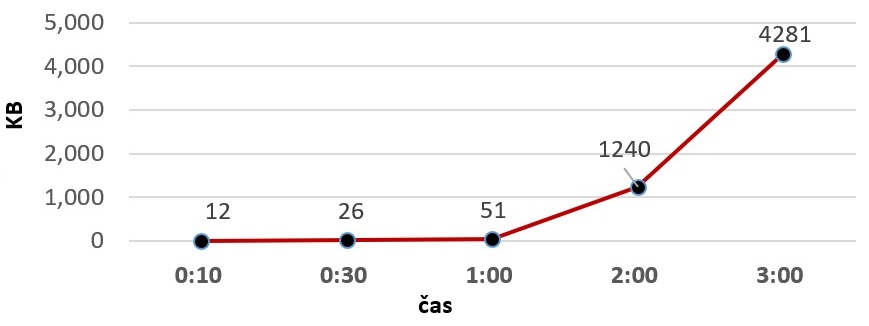
\includegraphics[width=0.7\textwidth]{Figures/graph2.jpg}\label{fig:buildingEscapeGraph2}
	\caption{Graf závislosti paměťového růstu na čase}
	\label{fig:buildingEscapeGraph2}
\end{figure}

Pro veškeré výpočetní operace s vektory byla vytvořena třída \textit{MyVector} z níž dědí třída \textit{MyVector2D}, která je využita pro pohyb davu v budově. První zmíněná je určená pro hejno. Důvod využití vlastní třídy je přenositelnost a nezávislost algoritmu na platformě. Všechny důležité třídy využívají k vytvoření scény pouze nativní knihovny C++.

Příklad ošetření jedné části kódu:

\begin{lstlisting}[language=c++,label=src:memory elimination,caption=Ukázka eliminace nárustu paměti]
this->tmpVector->set();
this->tmpVectorMem = this->tmpVector;
this->tmpVector = this->tmpVector->subTwoVector(location, Boidss->at(i)->location);
// ...operations with tmpVector
this->steer->addVector(this->tmpVector);
delete this->tmpVector;
this->tmpVector = this->tmpVectorMem;
\end{lstlisting}

Důležitý je třetí řádek, kdy se volá metoda \texttt{subTwoVector(...)}, která vrací výsledek odečtení dvou vektoru jako odkaz na nově vytvořenou paměť. Abychom zabránili nárustu paměti, musíme tento výpočet uložit do dočasné paměti \textit{tmpVector} se kterou provedeme patřičné operace a ve chvíli kdy jí už nebudeme potřebovat, tak ji smažeme.

Musíme však zachovat původní adresu \textit{tmpVector}. Pro tento účel slouží proměnná \\\textit{tmpVectorMem} která slouží jako prostředník pro uchování adresy. Pak tedy můžeme tuto původní adresu přiřadit zpět, v tomto případě poslední řádek kódu.
\\\\
Pro větší úsporu paměťi ve třídě \textit{Boids}, jejíž instance je volána v každé smyčce, tak jednotlivá pravidla i metody pro mezivýpočty používali mezi sebou stejné adresy pamětí.

Aby nedocházelo k neoprávněným přístupům a záměnou adres, tak byla využita pomocná proměnná do které se dočasně uložil výsledek pravidla a pak pomocí metody \texttt{set()} z~třídy \textit{MyVector} šlo bezpečně nastavil hodnoty vektoru bez jakéhokoliv úniku paměti. Tento způsob byl aplikován na všechna použitá pravidla, včetně vyhýbání se zdem.

Vůči 100 agentům ve scéně měla starší verze aplikace využití RAM 110 MB včetně použitých textur a objektů. Po těchto doposud zmíněných změnách bylo využití 91 MB.
\\\\
Další vylepšení bylo lepší použití cyklů. Klasický zápis cyklu který byl použit před tímto typem optimalizace je následujicí:
\begin{lstlisting}[language=c++,label=src:classic cycle,caption=Použití klasického cyklu] 
for (int i = 0; i < this->models->size(); i++) {...}
\end{lstlisting}
Dle oficiálních referencí pro C++ \cite{linkToCppReference} bylo zjištěno, že při každé iteraci cyklem se stále volá metoda \texttt{size()}, která tento výkon podstatně snižuje. Řešením je uložit tuto hodnotu do proměnné a tu pak  následně porovnávat v podmínce. Dalším vylepšením je použití prefixové inkrementace proměnné \textit{i}. Toto použití je mnohem účinnější než postfixová inkrementace z důvodu, že nepoužívá dočasné úložiště a vkládání potřebného kódu na pozadí \cite{linkToPreIncrementation}. Výsledný cyklus pak vypadá takto:
\begin{lstlisting}[language=c++,label=src:optimalized cycle,caption=Použití optimalizovaného cyklu] 
for (int i = 0, len = this->models->size(); i < len; ++i) {...}
\end{lstlisting}

Tyto změny důležitých cyklů v hlavní smyčce dokázaly přidat až 5 FPS.
\\\\
Další problém nastal v načítání objektů. Původní verze nahrávání objektů do scény probíhala\\ v obyčejné smyčce, takže stejné objekty \textit{(v tomto případě objekty agentů)} se načítali vícekrát. 

Řešení spočívalo v kopírovacím konstruktoru. Daný typ objektu byl načten pouze jednou a poté se v cyklu předávala adresa načteného objektu kopírovacímu konstruktoru, který tuto paměť nakopíroval pro svou instanci. Při načítání 100 agentů bylo celkově ušetřeno 40 sekund.

\begin{lstlisting}[language=c++,label=src:copy constructor,caption=Ukázka použití kopírovacího konstruktoru]
// loading object method in Flock class
Model *tmpBoidsModel = new Model(this->cfg->OBJ_BOID, this->cfg);
for (int i = 0; i < this->numberOfBoids; ++i) {
	if (tmpBoidsModel != NULL)
		this->boidsModel[i] = new Model(*tmpBoidsModel);
	}
}

// copy constructor in Model class
Model(const Model& model) 
: 
	textures_loaded(model.textures_loaded),
	meshes(model.meshes),
	directory(model.directory),
	gammaCorrection(model.gammaCorrection),
	cfg(model.cfg)
{}
\end{lstlisting}

\subsection{Steering behaviors}\label{sec:steering-behaviors}
Řízení chování \cite{linkToSteeringBehaviors} již zmíněné v teoretické části bylo použito pro reálnější podobu chování celého davu.

Jako první vlastnost byla použita metoda seek \textit{(hledání)} primárně použivané u Koheze při návratové hodnotě (viz kapitola \ref{sec:koheze} - kohezní síla), kde bylo upozorněno na složitější implementační část oproti zarovnání.

Hledání je určeno k tomu, aby agent směřoval k nějakému cíli, tak že upravuje aktuální rychlost \textit{(velocity)}. V případě koheze je cíl průměrná lokace okolních agentů. Výsledek této operace je seek vektor.

Následující kód ukazuje jak se seek vektor vypočítá.

\begin{lstlisting}[language=c++,label=src:seek,caption=Vypočtení seek vektoru]
this->tmpVectorMem = desired->subTwoVector(v, this->location);
this->desired->set(this->tmpVectorMem->vec.x, this->tmpVectorMem->vec.y, this->tmpVectorMem->vec.z);
delete this->tmpVectorMem;

this->desired->normalize();
this->desired->mulScalar(maxSpeed);

this->seekResult->set();
this->tmpVectorMem = seekResult->subTwoVector(this->desired, this->velocity);
this->seekResult->set(this->tmpVectorMem->vec.x, this->tmpVectorMem->vec.y, this->tmpVectorMem->vec.z);
delete this->tmpVectorMem;

seekResult->limit(maxForce);
\end{lstlisting}

Nejprve se spočte lokace na kterou má agent směřovat \textit{(vektor desired)}, a~nastavíme maximální zrychlení aby se na místo dostavil co nejdříve.

Následuje vypočtení samotného seek vektoru, který je roven rozdílu mezi požadovanou a~aktuální rychlostí. V poslední řadě pak musíme vektor limitovat konstantou tření \textit{(maxForce)}.
\\

Další vlastností která byla použita je následování bodů \textit{(Path Following)}. V této práci slouží jako následování kontrolních bodů v budově.

Po určení tohoto jednoho či více bodů na ně agent začně postupně směřovat. Při následování bodů se použivá funkce pro vypočtení seek vektoru, který je poté aplikován jako další pravidlo, tzn. k výsledné rychlosti se přičte další vektor (viz kapitola \ref{sec:aplikovani-tri-pravidel} - aplikování tří pravidel).

\newpage
\subsection{Třídní diagram}
Pro provoz simulace a chování davu slouží tři základní a tři pomocné třídy.

\begin{figure}[H]\centering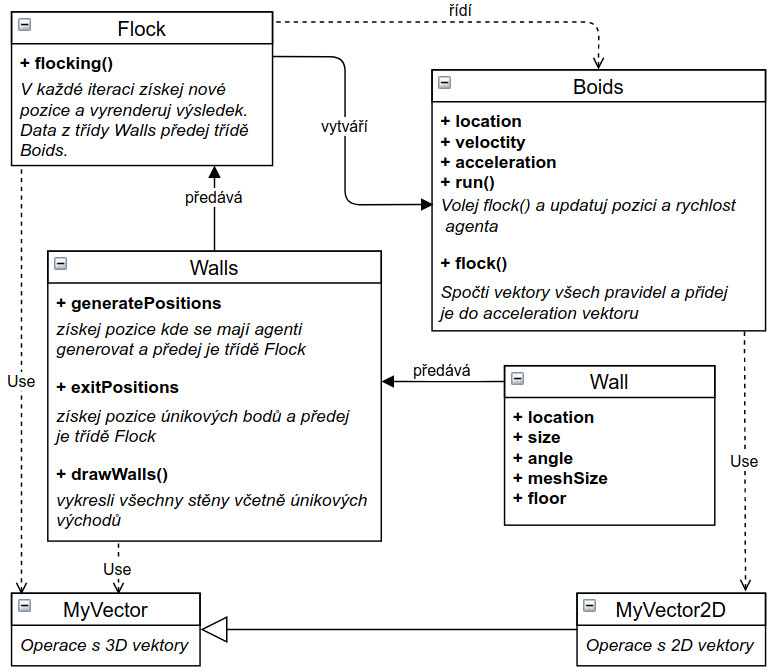
\includegraphics[width=0.8\textwidth]{Figures/diagram2.jpg}
	\caption{Diagram řídicích tříd}
\end{figure}

Hlavní třídou je třída Flock, která koordinuje komunikaci mezi třídou Walls a Boids. Zároveň se stará o veškeré vytváření agentů, kterým přiřažuje jednotlivé objekty ve scéně, jenž jsou vizualizovány uživateli. Také v každé iteraci volá simulační mechanismy pomocí metody \texttt{run()}.

Třída Walls vytváří zdi podle předaných dat z mapy a udržuje informace o generačních pozicích a pozicích únikových bodů. Díky tomu může třída Flock vygenerovat agenty do patřičného patra a pozice. Zároveň jsou tato data sdílena s třídou Boids, která může kontrolovat kolize se zdmi a počítat pozice únikových bodů na které má agent směřovat.

Jak již bylo zmíněno v kapitole \ref{sec:problemy-pri-implementaci}, tak pro operace s vektory byla použita vlastní třída \textit{MyVector} ze které dědí třída \textit{MyVector2D} z důvodu přenositelnosti a nezávislosti algoritmu na platformě.

\subsection{Výsledné aplikování pravidel}\label{sec:vysledne-aplikovani-pravidel}
Všechna pravidla jsou aplikována jako součet výsledků jednotlivých pravidel \textit{(viz kapitola \ref{sec:aplikovani-tri-pravidel} - aplikování tří pravidel)}. V této práci k sečtení a vytvoření výsledného vektoru slouží metoda \texttt{appplyForce(...))}, která přidá do výsledného vektoru \textit{acceleration} další vektor \textit{(výsledek jednoho z pravidel)}. Tento vektor je pak aplikován v metodě \texttt{update()}, která nastaví agentovi novou pozici a rychlost.

\begin{lstlisting}[language=c++,label=src:seek,caption=Nastavení výsledné pozice agenta] 
void Boids::update() {
	acceleration->mulScalar((float)(.4));
	velocity->addVector(acceleration);
	velocity->limit(maxSpeed);
	location->addVector(velocity);
	acceleration->mulScalar(0);
}
\end{lstlisting}

Po vynásobení konstantou 0.4, která slouží pro nastavení citlivosti \textit{(může a nemusí být použita, zde je nastavena po experimentech jako ideální)} následuje přidání, limitování vektoru a~vypočtení výsledné pozice. Na konci musíme vektor \textit{acceleration} vynulovat pro použití v další iteraci.

\subsection{Konfigurační soubor}
Konfigurační soubor je rozdělen do čtyř sekcí. První sekce se zaobírá nastavením základních parametrů jako pozice kamery, šířka či výška okna až po citlivost myši a nastevení scény \textit{(2D nebo 3D)}. 

Druhá sekce je zaměřena na únik z budovy, kdy se nastavují důležité parametry jako \\FLOOR\_TIME\_DURATION, který zajišťuje čas, po který daný agent sestupuje z patra, nebo \\PATH\_TO\_FIND\_RADIUS zajišťující velikost kruhu kolem únikového bodu. Pokud tedy bude kruh větší, agent začne dříve směrovat k druhému bodu.

Syntaxe souboru je následující:

\[JMENO\_PROMENNE=HODNOTA\]

Dále následuje celkové chování agentů jako rychlost, tření, počet agentů a počet objektů kterým se budou agenti vyhýbat. Toto nastavení má vliv na celkovou scénů nejvíce.

Třetí sekce nastavuje rychlost agentů, jejich velikost, velikost generačního pole ve kterém se agenti generují a hlavně důležitá pravidla jako velikost kruhu ve kterém se nachází agent se kterým bude iterovat či nastavení konstanty BOID\_DESIRED\_SEPARATION, která indikuje minimální vzdálenost agentů, kteří se přiblíží k sobě.

Čtvrtá sekce je zaměřena k načítání objektů do scény. Cesta, která se udává k objektu je relativní a tudíž objekt musí být umístěn v adresáři \textit{Models}, který se nachází na stejné adresářové úrovni jako výsledný spustitelný soubor \textit{Bachelor.exe}

Komentáře jsou řešeny jako ve výpisu níže:


\begin{lstlisting}[language=c++,label=src:seek,caption=Ukázka komentáře v konfiguračním souboru]
###############################################
# Section 2. 
# Building escape
###############################################
\end{lstlisting}

K označení řádku s komentářem indikujeme pomocí křížku, který  aplikace ignoruje. 

\subsection{Spuštění scény}\label{sec:spusteni-sceny}
Aplikaci lze spustit tak, že spustitelný soubor \textit{Boid.exe} přijímá jako první parametr jméno konfiguračního souboru a jako druhý parametr jméno textového souboru, ve kterém je uložené schéma budovy.

Pokud není uveden žádný z parametrů, aplikace načte konfiguraci ze souboru \textit{config.cfg} a~schéma budovy ze souboru \textit{map.txt}.

Pro dva typy scény \textit{(únik z budovy, simulace hejna ryb)} jsou připraveny dva konfigurační soubory: \textbf{configEscape.cfg} a \textbf{configFish.cfg}, které může uživatel modifikovat. 

K ukázce různých scén slouží soubory s příponou \textit{*.bat}, které spouštějí aplikaci s předem definovanými parametry. K výslednému programu jsou připraveny scény:

\begin{itemize}
	\item \textbf{boid\_escape\_variant\_1.bat} - varianta úniku z vícepatrové budovy, využívá schéma \\ze~souboru~\textit{map\_variant\_escape\_1.txt}
	\item \textbf{boid\_escape\_variant\_2.bat} - varianta úniku z vícepatrové budovy, využívá schéma \\ze~souboru~\textit{map\_variant\_escape\_2.txt}
	\item \textbf{boid\_labyrinth\_variant\_1.bat} - varianta úniku z labyrintu, využívá schéma \\ze~souboru~\textit{map\_variant\_labyrinth\_1.txt}
	\item \textbf{boid\_labyrinth\_variant\_2.bat} - varianta úniku z labyrintu, využívá schéma \\ze~souboru~\textit{map\_variant\_labyrinth\_2.txt}
	\item \textbf{boid\_fishes\_variant\_1.bat} - varianta hejna ryb s kolizním objektem kvádru \textit{(cube)}
	\item \textbf{boid\_fishes\_variant\_2.bat} - varianta hejna ryb s kolizním objektem sféry \textit{(sphere)}
\end{itemize}

Informace, které byly zaznamenány pro úniky z bodov různých typů, jsou zmíněné v kapitole \ref{sec:testovani-uniku-z-budovy} - testování úniku z budovy.
%Aplikaci lze spustit tak, že se jako první parametr načte jméno konfiguračního souboru. Pokud je první parametr prázdný, pak se načte obsah souboru \textit{config.cfg}. K adresáři \textit{Release} výsledné aplikace jsou přiloženy dva konfigurační soubory: \textit{configEscape.cfg} a \textit{configFish.cfg}, které jsou přiloženy jako parametry výsledného \textit{Bahelor.exe} souboru. Ke spuštění výsledných scén slouží soubory s příponou \textit{*.bat}, a sice \textit{fishes.bat} a \textit{escape.bat}. Připadně může uživatel měnit parametr názvu konfiguračního souboru spuštěním \textit{Bachelor.exe} z příkazové řádky.

%Pro testovací účely jsou pro uživatele vybrány tyto dva soubory, jejichž obsah parametrů konfiguračních souborů může modifikovat.

\subsection{Únik z budovy}\label{sec:unik-z-budovy}
První část využití Boidova agoritmu je simulace úniku lidí z budovy podle nastavených únikových cest. Funkčně je tato část určena k tomu, aby po skončení simulace mohl uživatel zjistit, kolik času by zabralo evakuovat lidi z předem definovaného plánu budovy. V případě časově náročné evakuace může uživatel upravit plán budovy a únikové cesty tak, aby budova splňovala dané normy.

Plán budovy můžeme upravovat v souboru \textit{map.txt}, případně využití vlastního schématu (viz kapitola \ref{sec:spusteni-sceny} - spuštění scény) včetně definování dalších pater a~únikových cest. Jelikož se jedná o~textový soubor, tak každý znak reprezentuje jinou funkci. Popis funkčních znaků můžeme vidět níže:

\begin{itemize}
	\item \textbf{G} generační místo pro dav, který lze použít vícekrát v každém patře či místnostech
	\item \textbf{-} reprezentuje vertikální stěnu
	\item \textbf{|} reprezentuje horizontální stěnu
	\item \textbf{+} reprezentuje spojovací stěnu jako kombinace horizontální a vertikální stěny
	\item \textbf{*} blok stěny jednoho bodu, proto ji lze použít jako reprezentaci sloupu v patře
	\item \textbf{=} reprezentuje začátek schématu nového patra
	\item \textbf{/} ukončovací znak schématu patra
	\item \textbf{A-Z, a-z} únikové body podle který se dav řídí \textit{(mimo G jako generační bod a F jako ukončovací bod zřetězeného řízení davu, viz níže)}
	\item \textbf{1-9, F} zřetězené řízení davu použité jako únik z labyrintu pomocí 10 únikových bodů
\end{itemize}

Pro únik v jedné části budovy jsou požity dva znaky \textit{(např.: velké  písmeno A a malé a)}. Nejdříve dav směřuje k menšímu znaku a poté k většímu, který indikuje finální bod. V každém patře může být těchto únikových bodů libovolný počet, kdy pokud v jednom patře končíme např.: znakem D, pak se v dalším patře začíná od znaku E. Jenotlivý agent určuje ke kterému bodu jít pomocí vzdálenosti od něj \textit{(tj. k nejbližšímu)}.

Druhým typem úniku je únik z labyrintu, tedy složitějších prostor budovy kdy je potřeba více než dva únikové body. Dav začne směřovat k nejbližšímu nejmenšímu číslu a pokud tohoto čísla dosáhne, tak poté začne směřovat k dalšímu o 1 větší dokud neskončí u písmene F. Tento způsob lze aplikovat pouze u vykreslení jednoho patra. 
\\\\
Při spuštění aplikace, která vykreslí definované schéma lze scénu ovládat pomocí následujících kláves:

\begin{itemize}
	\item \textbf{1-9} klávesou lze přepínat mezi pohledy jednotlivých pater, přičemž se neaktuální patro přepne do režimu průhlednosti
	\item \textbf{E} přepnutí celé budovy do řežimu průhlednosti se zvýrazněním davů
	\item \textbf{Q} opětovné vykreslení celé budovy bez režimu průhlednosti pater
	\item \textbf{F} přepnutí do režimu celé obrazovky, opětovným stiskem lze aplikaci přepnout zpět do režimu okna
	\item \textbf{Mezerník} spuštění simulace, opětovným stiskem lze simulaci ukončit
\end{itemize}

Výslednou scénu lze přepnout do fullscreen režimu pomocí klávesy F případně zpět.

\begin{figure}[H]
	\centering
	\subfloat[ Půdorys]{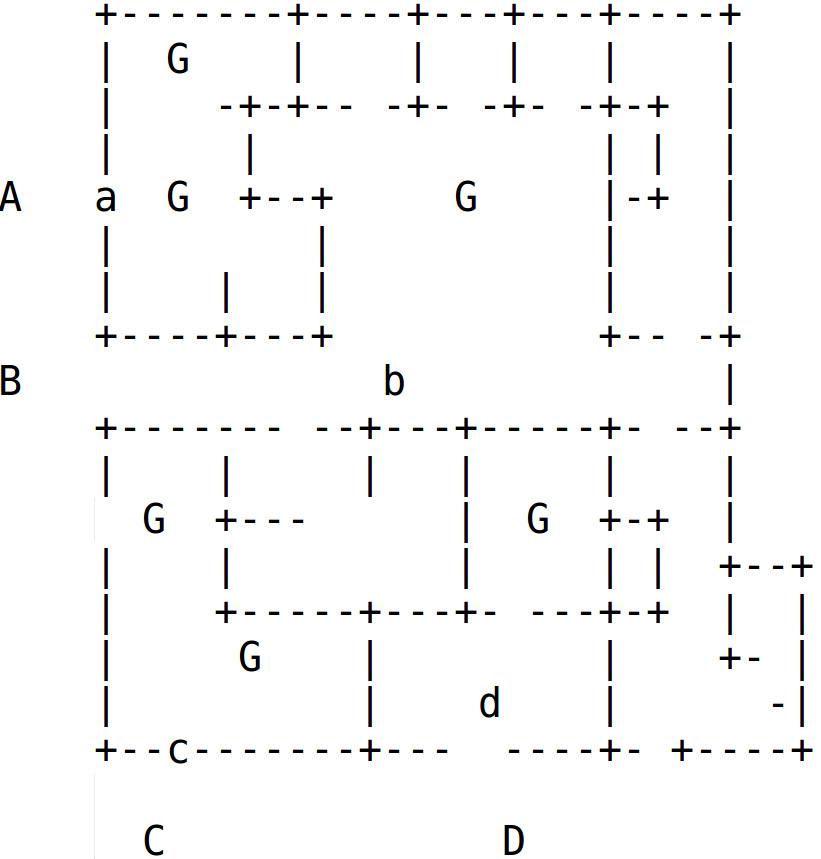
\includegraphics[width=0.43\textwidth]{Figures/map3.jpg}\label{fig:mapatxt}}
	\hfill
	\subfloat[ Patro]{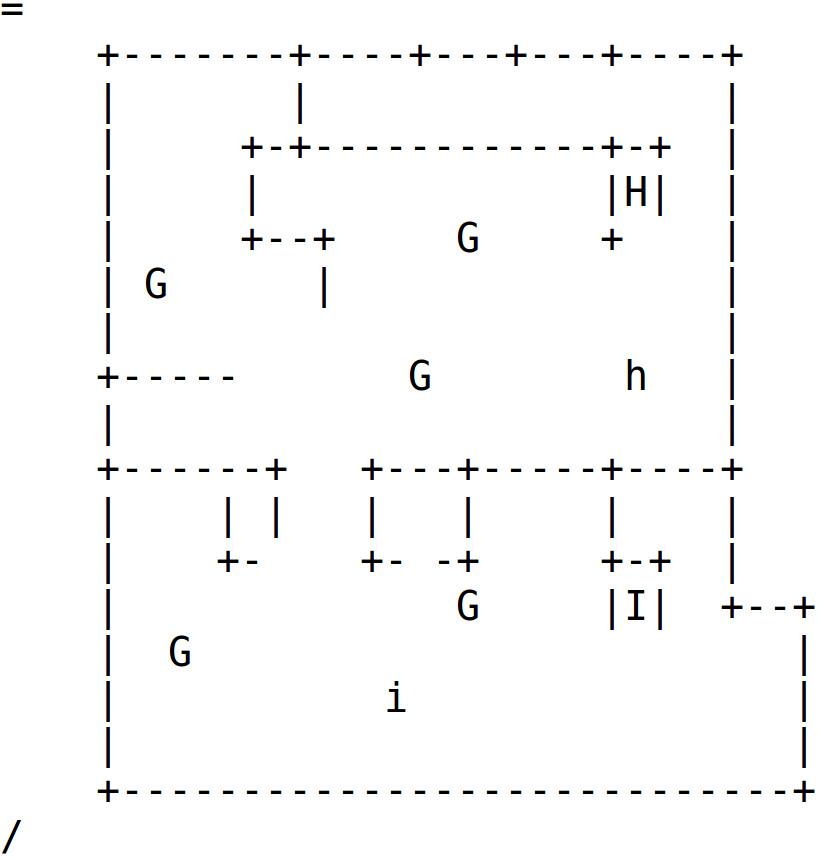
\includegraphics[width=0.43\textwidth]{Figures/map4.jpg}\label{fig:mapatxt}}
	\caption{Ukázka nákresu budovy v textovém souboru} \label{fig:mapatxt}
\end{figure}

		%\begin{Verbatim}[baselinestretch=0.8]
	
		%\end{Verbatim}



Při zapnutí simulace jsou agenti v půdorysu okamžitě vedení směrem ven mimo budovu, avšak agenti v dalších patrech musí využít jiné evakuační cesty aby se dostali do spodního patra odkud můžou vyjít ven\footnote{Agenty v patře lze také směrovat rovnou ven mimo budovu, tj.~forma venkovního evakuačního schodiště. Dole v přízemí mimo budovu však musí být definován další evakuační bod (pod ``schodištěm''), jinak začnou agenti směřovat k nejbližšímu bodu, který by jinak byl v budově.}. Proto pokud se agent v patře dostane k finálnímu bodu úniku \textit{(velké písmeno)}, začne ``sestupovat'' do přízemí budovy. Sestup však zabere nějaký čas, jednak kvůli zatížení únikových cest tak samotného sestupu. Souvisí s tím také to, že agentovi v posledním patře bude sestup trvat déle než agentovi v prvním patře. Hodnotu míry opuštění budovy \textit{(konkrétněji: evakuační výtah je rychlejší než evakuační schodiště)} lze měnit v konfiguračním souboru pomocí konstanty FLOOR\_TIME\_DURATION.

\begin{figure}[H]\centering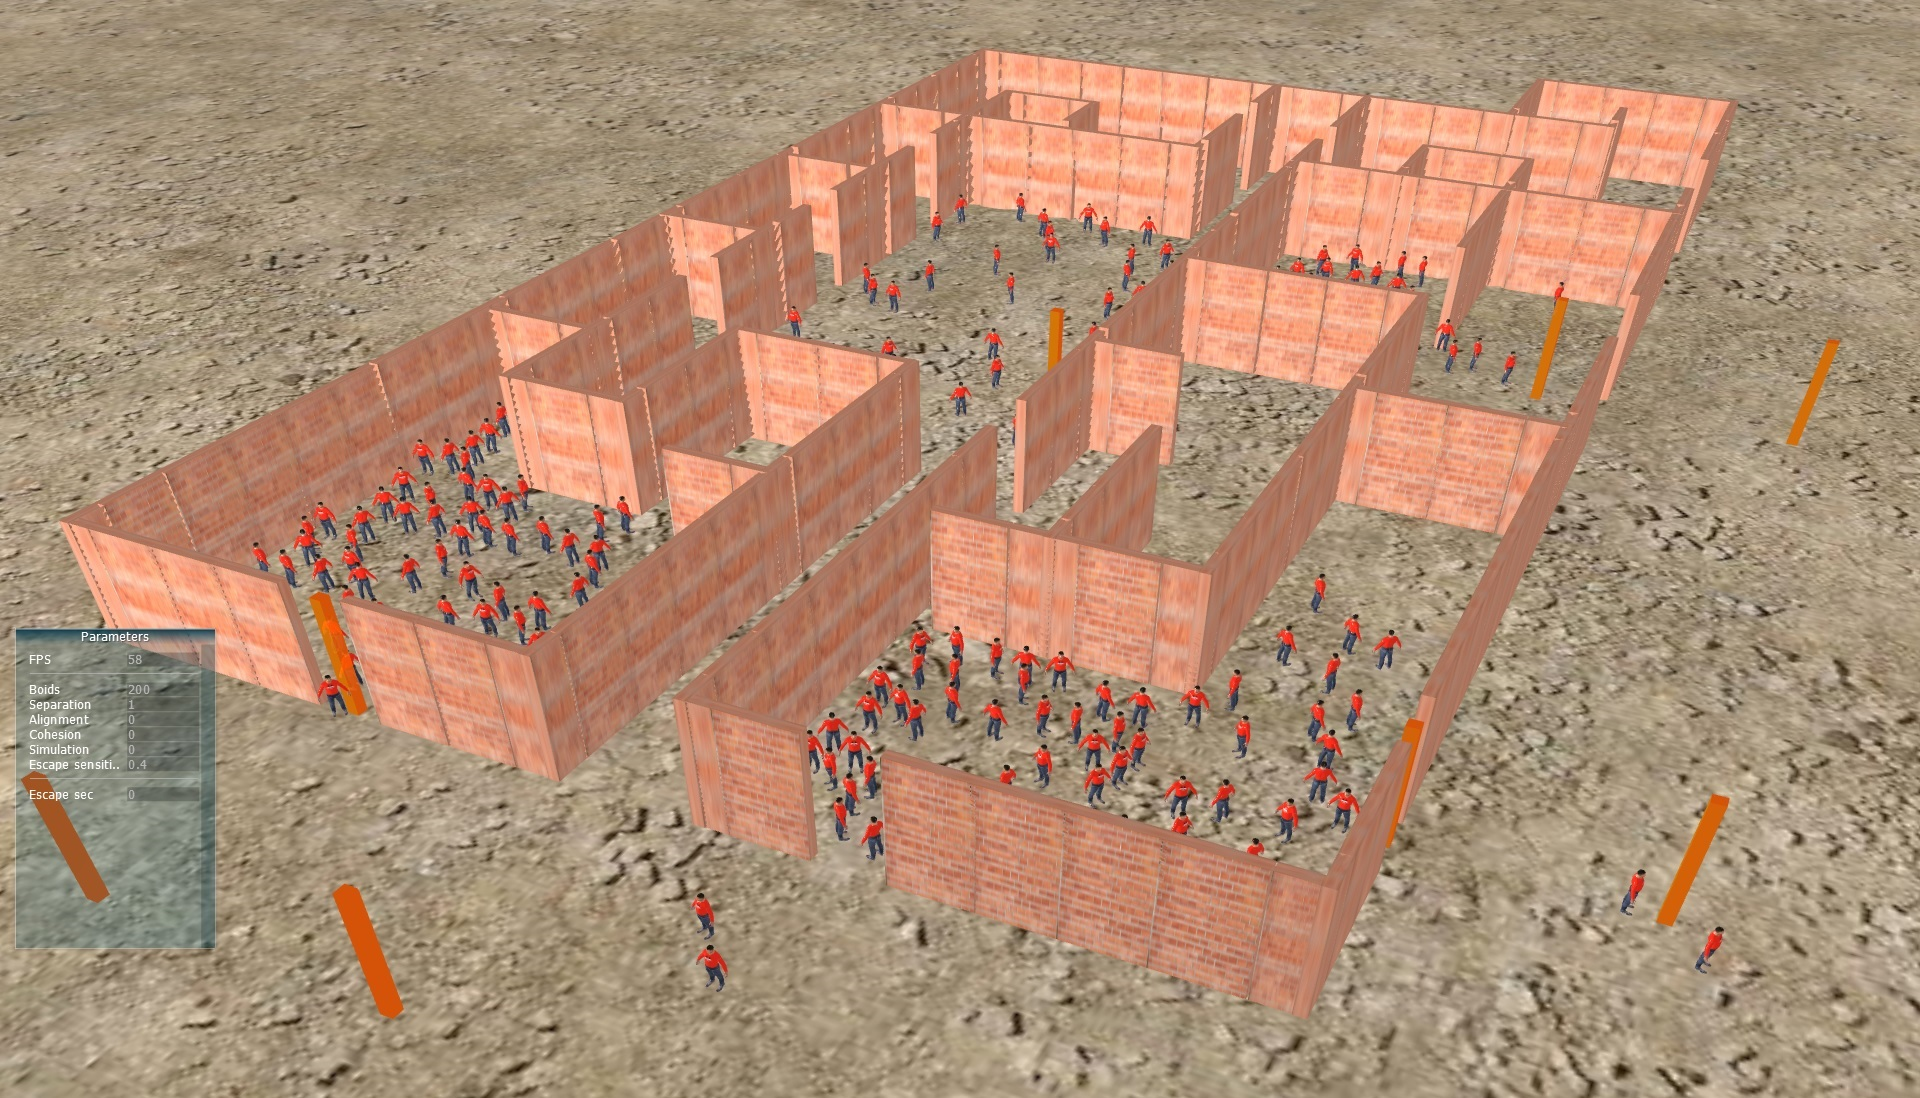
\includegraphics[width=0.66\textwidth]{Figures/screen9.jpg}
	\caption{Ukázka vyrenderovaného půdorysu budovy}
\end{figure}

Pro následování bodů byla použita metoda \texttt{arriveTo(...)} která využívá metodu \texttt{seek(...)} \textit{(viz kapitola \ref{sec:steering-behaviors} - steering behaviors)}. Abychom správně určili, který agent má kam směřovat, musíme metodě\\\texttt{arriveTo(...)} předat správný vektor, který získáme metodou \texttt{getArriveVector(...)}. Ta vrátí výsledný vektor který je předán \texttt{seek()} metodě. Výsledek je pak nový vektor, který se aplikuje jako nové pravidlo \textit{(viz kapitola \ref{sec:aplikovani-tri-pravidel} - aplikování tří pravidel)} a~tím zajistíme že agent bude směřovat na nejbližší únikový bod a~následně na finální bod. 

\begin{lstlisting}[language=c++,label=src:mapSave,caption=Princip metody getArriveVector(...)]
// getting minIndex from exitPoints...
if ((walls->exitPositions.at(minIndex)->vec.y / walls->floorDiferencial) == this->floor) {
	
	if (location->distance(walls->exitPositions.at(minIndex)) < cfg->PATH_TO_FIND_RADIUS && !this->incrementedOnce) {
		++minIndex;
		this->incrementedOnce = true;
	}
	// code...
	return walls->exitPositions.at(minIndex);
}
\end{lstlisting}

V první části kódu, zde nezmíněné kvůli délce, je získání \textit{minIndex} hodnoty ve které je uložen index z kontejneru \textit{map}, odkud začínají souřadnice únikových bodů ve stejném patře jako je aktuálně kontrolovaný agent. Pokud tedy v půdorysu bude 8 únikových bodů, jak je zobrazeno na obrázku č. \ref{fig:mapatxt}, tj. 4 finální únikové cesty, pak \textit{minIndex} v následujícím patře bude 9. Je třeba upozornit, že hodnota \textit{minIndex} vždy odkazuje na index menšího písmena.

Následuje podmínka jenž kontroluje, zda-li se agent nachází ve stejém patře jako únikový bod \textit{(souřadnice Y únikového bodu vydělená výškou jednoho patra - konstanta třídy Walls)} a~následná kontrola, zda se agent dostal do blízkosti okruhu únikového bodu. Pokud ano, může agent pokračovat k finálnímu bodu tak, že hodnotu \textit{minIndex} zvýšíme o 1.

Mimo další operace které se nachází mezi návratovou hodnotou a předchozími podmínkami, je nakonec vrácen vektor s indexem \textit{minIndex}.

Útěk ze složitějších prostor pomocí čísel \textit{(útěk z labyrintu)} funguje na stejné bázi s~tím rozdílem, že se hodnota inkrementuje do té doby dokud agent nenarazí na písmeno F, čili koncový bod.

\subsubsection{Problémy při úniku z budovy}\label{sec:problemy-pri-uniku-z-budovy}

Agenti se můžou občas dostat do problémů zejména díky špatnému návrhu budovy, nebo také kvůli nedokonalosti Boidova algoritmu. 

Například pokud při úniku z budovy zapneme všechna tři pravidla \textit{(separace, zarovnání, koheze)}, může nastat efekt procházení zdí. Tento problém vzniká kvůli nastaveným konstantám citlivosti u každého pravidla. Tyto konstanty byly nastaveny po řadě experimentů jako nejvhodnější a~jsou neměnné \textit{(kromě konstanty citlivosti úniku ESCAPE\_SENSITIVITY, kterou lze měnit v konfiguračním souboru)}. Pokud je konstanta příliš nízká, dané pravidlo by zaniklo mezi ostatními. Pokud příliš vysoká, tak by dané pravidlo překrylo ostatní. U konstanty citlivosti úniku je však občas potřebné přenastavení. Částečné řešení spočívá jen v použití separace. Dav se tedy chová jako dav skutečných lidí \textit{(každý si jde kam chce)}.

Další problém může nastat při generování agentů, kdy agenti vyberou jako cestu \\k nejkratšímu bodu tu variantu, že se bod nachází za zdí či v jiné místnosti (viz obrázek č. \ref{fig:buildingEscapeProblem1}). S tím souvisí možnost zaseknutí o zeď, kdy má agent před sebou překážku za kterou je cílový bod a např.: dva bloky od něj je východ. Má však nastavenou cestu přímo na bod \textit{(přes zeď)}.

S generováním souvisí ještě jedna věc, a sice při generování většího množství agentů na malém prostoru se může některý z nich ``zabořit'' do zdi a už se z ní nemůže dostat. 

\begin{figure}[H]\centering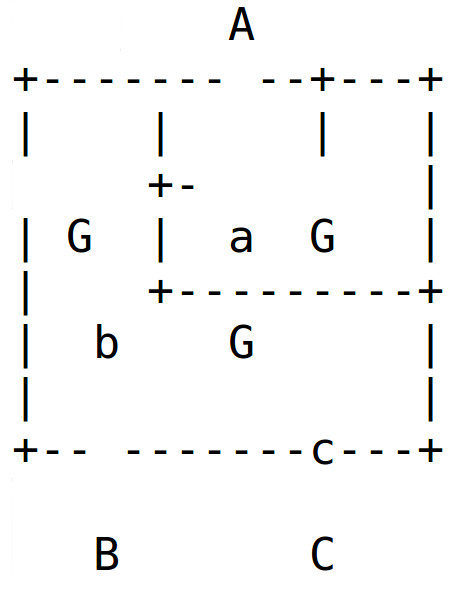
\includegraphics[width=0.25\textwidth]{Figures/buildingEscapeProblem2.jpg}\label{fig:buildingEscapeProblem1}
	\caption{Problém uváznutí při špatném určení únikových bodů}
	\label{fig:buildingEscapeProblem1}
\end{figure}

Dále můžou nastat problémy při úniku ze složitějších prostor \textit{(labyrintu)}, kde uživatel nastaví číslo úniku u hrany stěny o kterou se může agent zaseknout. V případě většího davu \textit{(okolo 300 lidí)} a úzkých prostor můžou být ti, kteří splinili podmínku a dostali se k bodu, ``vytlačeni'' ostatními přes zeď a tím se dostat do situace že následující bod se nachází za zdí. 

V neposlední řadě s výše zmíněným problém může nastat situce, že je agent úspěšně ``vytlačen'', ale vrací se zpět na předchozí bod, který kvůli předešlé vysoké koncetraci agentů němel označen jako splněný. Částečné řešení spočívá v nastavení konstanty velikosti kruhu kolem únikového bodu pomocí konstanty PATH\_TO\_FIND\_RADIUS.
\subsection{Testování úniku z budovy}\label{sec:testovani-uniku-z-budovy}

Testování proběhlo na PC s parametry: CPU Intel i5-2500 @ 3.3GHz, grafická karta Radeon R9 280X Dual-X, RAM 12GB. Hodnoty se můžou na jiných PC lišit.


%\begin{table}[H]
%	\centering
%	\caption{Tabulka parametrů PC na kterých proběhlo testování}
%	\label{tab:tablepc}
%	\renewcommand{\arraystretch}{1.0}
%	\begin{tabular}{| c | c | c | c |}
%		\hline
%		& PC1 & PC2 & PC3 \\\hline
%		CPU & Intel i7-2637M @ 2.7GHz & Intel i5-2500 @ 3.3GHz& Intel i7-5820 @ 3.3GHz\\
%		RAM & 4 GB & 12 GB & 16 GB\\
%		GPU & Intel HD Graphics 3000 & Radeon R9 280X Dual-X & GeForce 1070 Ti\\
%		\hline
%	\end{tabular}
%\end{table}

Všechny části testů byly provedeny na schématech budov s parcelami první budovy 30x17 bloků a~druhé budovy 30x21, kdy jeden blok odpovídá jednomu znaku v textovém souboru, ve kterém je definováno schéma budovy, a~na 1x1 blok se vejde průměrně 5~agentů bez větších kolizí.

Tabulka zobrazuje jaké byly hodnoty FPS při daném počtu agentů, počtu pater a složitosti budovy \textit{(počet zdí)}. Hodnoty FPS jsou odečteny před a během simulace. Poslední hodnotou je čas opuštění budovy.

%Testy proběhly při počtu agentů 200, počtu pater 5, rychlostí agentů 3 s maximální hodnotou tření 0.1 a nastavení míry opuštění jednoho patra na 8 sekund.

První část testů proběhla nad schématem budovy, které je dostupné ve výsledném adresáři v~souboru s~názvem \textit{map\_variant\_escape\_1.txt}.

Testy proběhly při natavených hodnotách:

\begin{itemize}
	\item počtu agentů 200
	\item rychlostí agentů 3
	\item maximální hodnotou tření 0.1 
	\item míra opuštění jednoho patra na 8 sekund
\end{itemize}

%\begin{table}[H]
%	\centering
%	\caption{Tabulka naměřených hodnot - PC1}
%	\label{tab:tablePC1}
%	\renewcommand{\arraystretch}{1.0}
%	\begin{tabular}{| c | c | c | c | c | c |}
%		\hline
%		Pater  & Únikových bodů & Počet zdí & FPS před & FPS během & Čas [s]\\\hline
%		0 & 8 & 193 & 51 & 50 & 65.3\\
%		1 & 10 & 343 & 48 & 46 & 151.6\\
%		2 & 14 & 513 & 43 & 40 & 202.1\\
%		3 & 18 & 683 & 39 & 37 & 213.7\\
%		4 & 22 & 853 & 36 & 31 & 245.2\\
%		5 & 24 & 1023 & 32 & 28 & 337.1\\
%		\hline
%	\end{tabular}
%\end{table}

\begin{table}[H]
	\centering
	\caption{Tabulka naměřených hodnot - schéma 1}
	\label{tab:tableTesting1}
	\renewcommand{\arraystretch}{1.0}
	\begin{tabular}{| c | c | c | c | c | c |}
		\hline
		Pater  & Únikových bodů & Počet zdí & FPS před & FPS během & Čas [s]\\\hline
		0 & 8 & 193 & 56 & 55 & 61.6\\
		1 & 10 & 343 & 57 & 55 & 121.7\\
		2 & 14 & 513 & 52 & 45 & 153.1\\
		3 & 18 & 683 & 46 & 38 & 162.4\\
		4 & 22 & 853 & 41 & 39 & 173.3\\
		5 & 24 & 1023 & 40 & 36 & 246.5\\
		\hline
	\end{tabular}
\end{table}

Výsledné hodnoty jsou závislé zejména na dvou konstantách a sice ESCAPE\_SENSITIVITY, která udává přímočarost následování dalšího bodu a PATH\_TO\_FIND\_RADIUS, která indikuje velikost radiusu do kterého pokud se agent přiblíží, přesměruje se na další bod.
\\
\\
Další testy proběhly nad schématem uloženého v souboru \textit{map\_variant\_escape\_2.txt}.

\begin{table}[H]
	\centering
	\caption{Tabulka naměřených hodnot - schéma 2}
	\label{tab:tableTesting2}
	\renewcommand{\arraystretch}{1.0}
	\begin{tabular}{| c | c | c | c | c | c |}
		\hline
		Pater  & Únikových bodů & Počet zdí & FPS před & FPS během & Čas [s]\\\hline
		0 & 8 & 172 & 102 & 99 & 57.5\\
		1 & 10 & 362 & 86 &  84 & 235.2\\
		2 & 16 & 547 & 57 & 57 & 186.6\\
		3 & 22 & 732 & 46 & 38 & 164.5\\
		4 & 28 & 917 & 49 & 49 & 170.9\\
		5 & 34 & 1102 & 44 & 43 & 169.1\\
		\hline
	\end{tabular}
\end{table}

Kompletní plány budov lze nalézt v souborech: \textit{map\_completed\_variant\_1.txt} \\a \textit{map\_completed\_variant\_1.txt}.

Jak je patrné z grafu na obrázku č. \ref{fig:buildingEscapeGraph}, tak v prvním patře druhého schématu byl únik z~budovy časově náročnější z důvodu použití jednoho únikového bodu. Dále však bylo toto schéma, co se času úniku týče lepší, neboť schéma obsahuje jednodušší prostory budovy a~lepší návrhy únikových bodů.

\begin{figure}[H]\centering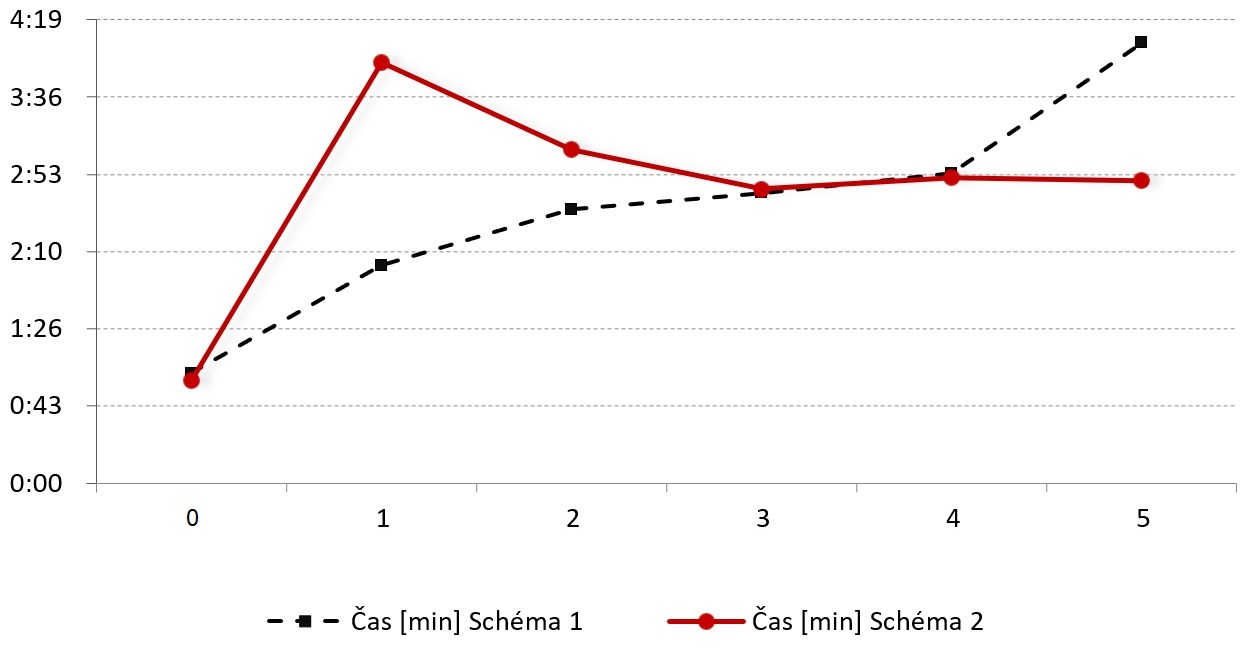
\includegraphics[width=0.75\textwidth]{Figures/graph.jpg}\label{fig:buildingEscapeGraph}
	\caption{Graf závislosti času úniku na počtu pater }
	\label{fig:buildingEscapeGraph}
\end{figure}

Další části testování proběhly nad složitějšími prostory bodovy o parcele 23x12. Jak již bylo zmíněno v kapitole \ref{sec:unik-z-budovy} - únik z budovy, tak úník z labyrintu \textit{(složitějších prostor)} funguje na principu umisťování čísel do mapy, kdy agenti směřují od nejmenší po největší číslo a následně k finálnímu bodu F.
\begin{figure}[H]\centering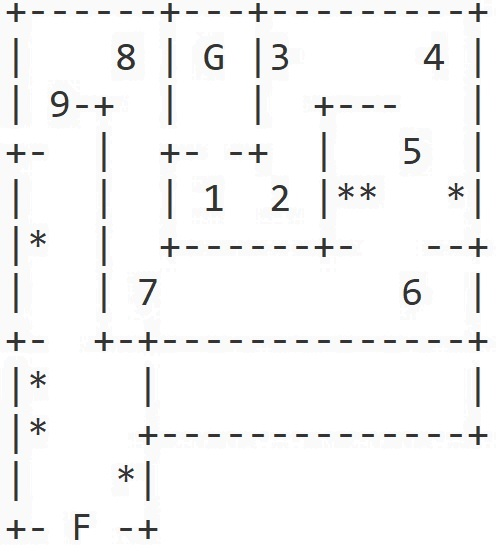
\includegraphics[width=0.35\textwidth]{Figures/map6.jpg}\label{fig:labyrinth}
	\caption{Ukázka nákresu labyrintu}
	\label{fig:labyrinth}
\end{figure}

Testování času úníku proběhlo na schématu, které můžeme vidět na obrázku č. \ref{fig:labyrinth}, při nastavené rychlosti na 1.5 a tření na 0.1. Srovnání výsledků s jinými patry však nelze zrealizovat, protože u této metody lze použít pouze jedno patro. 

\begin{table}[H]
	\centering
	\caption{Tabulka naměřených hodnot - labyrint}
	\label{tab:tablePC2}
	\renewcommand{\arraystretch}{1.0}
	\begin{tabular}{| c | c | c | c | c | c |}
		\hline
		Počet agentů & FPS před & FPS během & Čas [s]\\\hline
		20 & 280 & 279 & 46.4\\
		30 & 275 & 265 & 51.8\\
		40 & 267 & 261 & 63.2\\
		50 & 260 & 245 & 74.6\\
		\hline
	\end{tabular}
\end{table}

U této metody je také potřeba opomenout nastavení konstanty PATH\_TO\_FIND\_RADIUS. Pokud je radius větší, agent splní podmínku dosažení bodu když bude dále od něj. Toto nastavení je vhodné zejména pro větší prostory budov z~důvodu eliminace přímočarého pohybu k~únikovým bodům.

Ve výsledném adresáři jsou připraveny soubory \textit{boid\_labyrinth\_variant\_1.bat} \\a \textit{boid\_labyrinth\_variant\_2.bat}, kdy první zmíněný spouští scénu s početem agentů 20 a~druhý s~početem 50. Při spuštění druhé varianty lze spatřit efekt zaboření do zdi, případně vytlačení agenta ostatními, díky velkému počtu agentů na malém prostoru, zmíněné v kapitole\\ \ref{sec:problemy-pri-uniku-z-budovy}~-~problémy při úniku z budovy.

\newpage

%\begin{figure}[H]
%	\centering
%	\subfloat[Jednodušší labyrint]{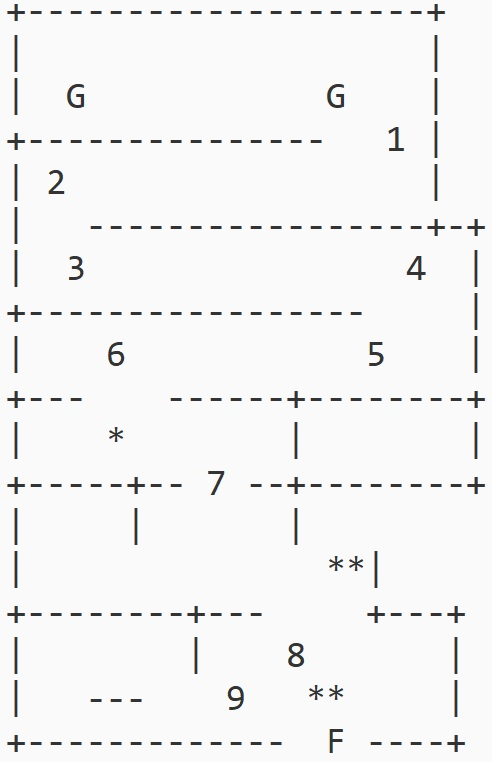
\includegraphics[width=0.3\textwidth]{Figures/map5.jpg}\label{fig:mapalabyrinth}}
%	\hfill
%	\subfloat[Složitější labyrint]{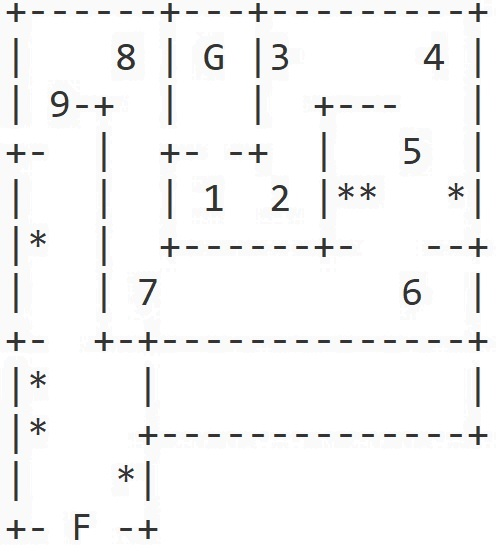
\includegraphics[width=0.35\textwidth]{Figures/map6.jpg}\label{fig:mapalabyrinth}}
%	\caption{Ukázka nákresu dvou labyrintů} \label{fig:mapalabyrinth}
%\end{figure}

%\begin{table}[H]
%	\centering
%	\caption{Tabulka naměřených hodnot - PC3}
%	\label{tab:tablePC3}
%	\renewcommand{\arraystretch}{1.0}
%	\begin{tabular}{| c | c | c | c | c | c |}
%		\hline
%		Pater  & Únikových bodů & Počet zdí & FPS před & FPS během & Čas [s]\\\hline
%		0 & 8 & 193 & 120 & 118 & 58.2\\
%		1 & 10 & 343 & 111 & 105 & 94.1\\
%		2 & 14 & 513 & 102 & 92 & 97.3\\
%		3 & 18 & 683 & 90 & 84 & 112.4\\
%		4 & 22 & 853 & 82 & 71 & 116.1\\
%		5 & 24 & 1023 & 74 & 64 & 169.8\\
%		\hline
%	\end{tabular}
%\end{table}

%Jak je patrné, tak čím více je pater, tím více klesá FPS z důvodu více kontrol kolizí se zdmi \\\textit{(i když se řeší kolize v každém patře zvlášť)}.

\newpage

\subsection{Simulace hejna ryb}
Druhý typ využití Boidova algoritmu je simulace hejna. V tomto případě je použita simulace ryb, ale při změně načítaného objektu v konfiguračním souboru můžeme vytvořit simulaci hejna čehokoliv. Pro změnu scény je třeba přepsat několik parametrů, zejména pak SCENE\_TYPE na 3D. U výsledné aplikace je připraven obsah souboru \textit{configFish.cfg} pro simulaci ryb. Pro výslednou scénu byly připraveny jednotlivé varianty (viz kapitola \ref{sec:spusteni-sceny} - spuštění scény)

Algoritmus funguje stejně jako při úniku z budovy, výjma využití třídy \textit{MyVector2D}, která je nahrazena výpočty ve 3D třídou předka \textit{MyVector}.

V konfiguračním souboru můžeme nastavit počet objektů, kterým se agenti budou vyhýbat. V případě, že se agent dostane do blízkosti objektu, pak vyhýbání funguje obdobně jako separace, akorát normalizování vektoru a vydělení vektoru počtem okolních agentů je nahrazeno vynásobení skalárem. Můžeme také nastavit útvar, ve kterém se budou agenti pohybovat. Na výběr je sféra \textit{(sphere)}, nebo kvádr \textit{(cube)} nastavitelné pomocí konstanty BOID\_SPACE\_TYPE.

\begin{figure}[H]\centering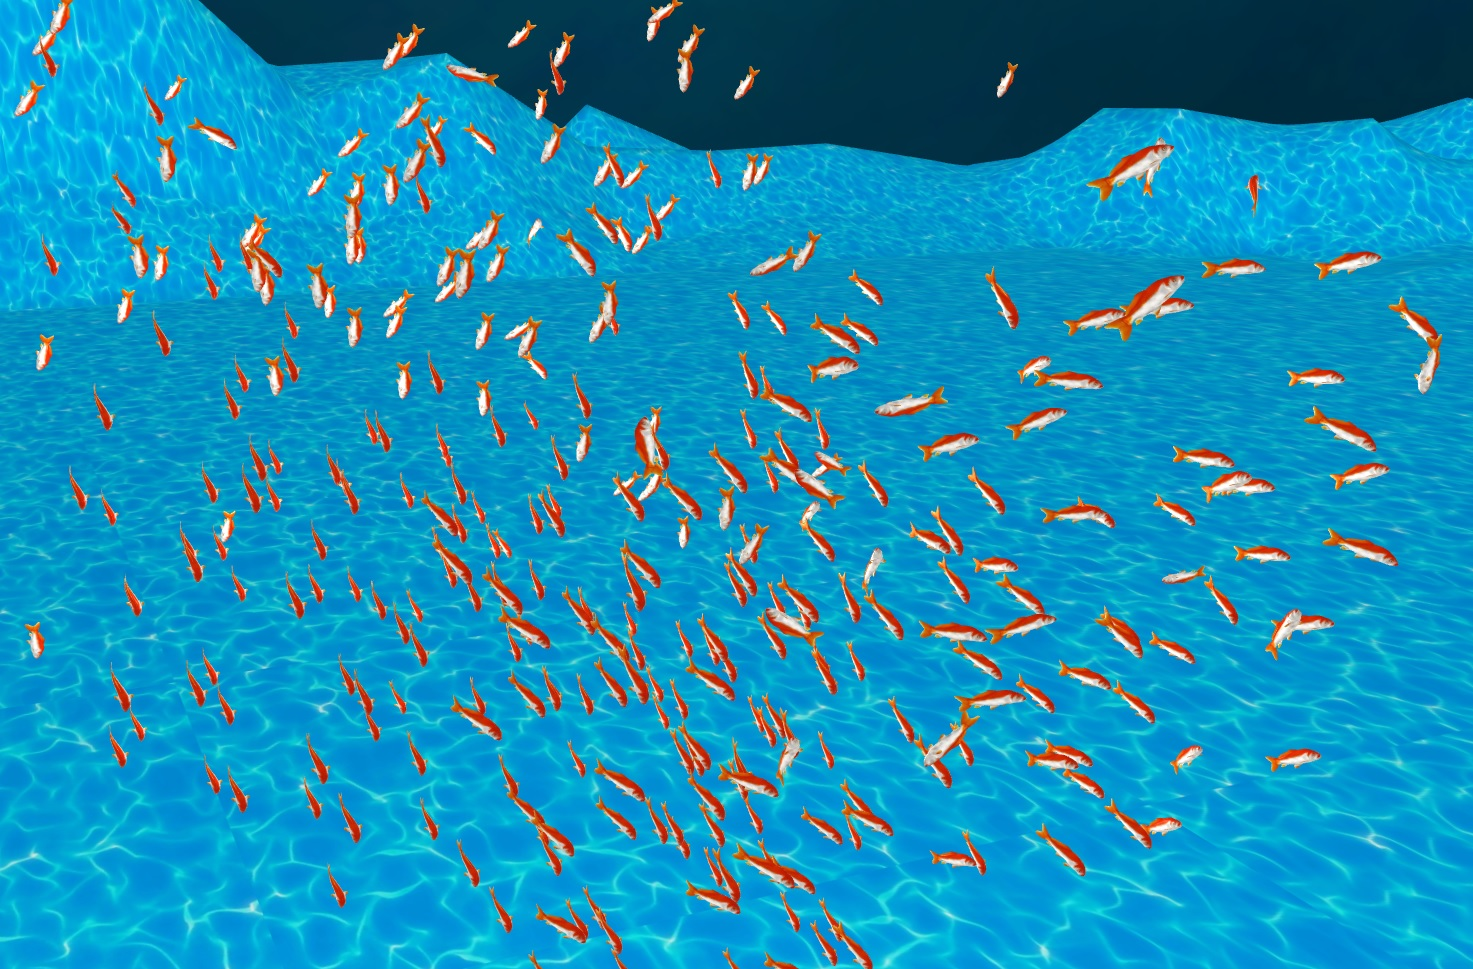
\includegraphics[width=0.7\textwidth]{Figures/new_fish3.jpg}\label{fig:fishExample}
	\caption{Ukázka hejna ryb}
	\label{fig:fishExample}
\end{figure}

%U této simulace jsou hodnoty FPS přijatelné i pro slabší PC, tj. pro již zmíněné hodnoty v~tabulce č. \ref{tab:tablepc} byly hodnoty pro PC1 a PC2 cca 65 FPS a~to při počtu agentů 400.

U této simulace je průměrná hodnota FPS 65 s počtem agentů 400 při parametrech PC zmíněných v kapitole \ref{sec:testovani-uniku-z-budovy} - testování úniku z budovy.

\subsubsection{Problémy při simulaci hejna}\label{sec:problemy-pri-simulace-hejna}
U této simulace nastávají problémy ``cukání'' pokud agent začne vyhodnocovat, že se přiblížil k~okraji mapy. Důvod tohoto efektu je aplikování kolize s ostatními agenty a zároveň kolize s~okrajem mapy. Tento problém byl zmírněn při nastavení různých citlivostí jednotlivých pravidel.

Pro menší množství agentů \textit{(např.: 20 agentů na větší ploše)}, nebyl tento efekt tak viditelný, jako při vizualzaci několika set agentů.

Nějvětší problémy nastávaly při nastavování konstant jako např: konstanty pro jednotlivá pravidla, kdy při špatném nastavení pohybu agentů chování neodpovídalo realitě.

\newpage
\section{Zhodnocení}

%Z výsledků tabulek č. \ref{tab:tablePC1}, \ref{tab:tablePC2} a \ref{tab:tablePC3} je znatelné, že pokud je PC výkonější pak čas úniku je kratší. Toto však lze zobecnit stejnými časy díky nastavení rychlosti agentů. U PC2 byla rychlost agentů vizuálně nejblíže, kdežto u PC3 agenti ``utíkali'' z budovy nepřirozeně rychle a u PC1 šli krokovým tempem. Lze tedy říci, že realitě nejvíce odpovídají hodnoty z tabulky pro PC2.

I když byly použity vylepšené techniky Boidova algoritmu (seek, path following) a~vyladěná všechna tři pravidla (separace, zarovnání, koheze), tak stále tento algoritmus není dokonalý (kapitoly \ref{sec:problemy-pri-uniku-z-budovy} - problémy při úniku z budovy, \ref{sec:problemy-pri-simulace-hejna} - problémy při simulaci hejna). Jako hlavní problém byl vyhodnocen stav, kdy se v dané scéně musí nastavit důležité konstaty (viz níže) citlivosti tak, aby pohyb agentů byl reálný.

Největší problémy nastavování konstant citlivostí, konkrétněji pěti hlavních (citlivosti jednotlivých tří pravidel, vyhýbání se okraje kolizních zdí a celková citlivost v metodě \texttt{update()}, viz kapitola \ref{sec:vysledne-aplikovani-pravidel} - výsledné aplikování pravidel), nastávaly u scény se simulací hejna ryb, kdy při špatném nastavení konstant byl pohyb přímočarý, tzn: změna směrového vektoru byla provedena okamžitě a ne plynule.
%Do budoucna by bylo vhodné tato pravidla dodělat a~tím zajistit, aby agenti v~budově byli inteligentnější a~nešli přímou cestou za únikovým bodem, ale mohli se rozhodovat o úniku dle sektorů budovy.

I přes tyto nedostatky lze Boidův algoritmus efektivně aplikovat jako simulaci jakéhokoliv hejna (v této práci hejna ryb viditelné na obrázku č. \ref{fig:hejnoRyb}), což je také nejvyužitelnější způsob. 
%Přesto je díky své nedokonalosti a zároveň jednoduchosti nejpoužívanějším algoritmem pro simulaci davu na bázi AI.

%Tento algoritmus je tedy plně využitelný jak ve filmovém tak v herním průmyslu v široké škále odvětví od simulace hejna ptáků po simulaci ryb v moři. 

\newpage

\begin{figure}[H]\centering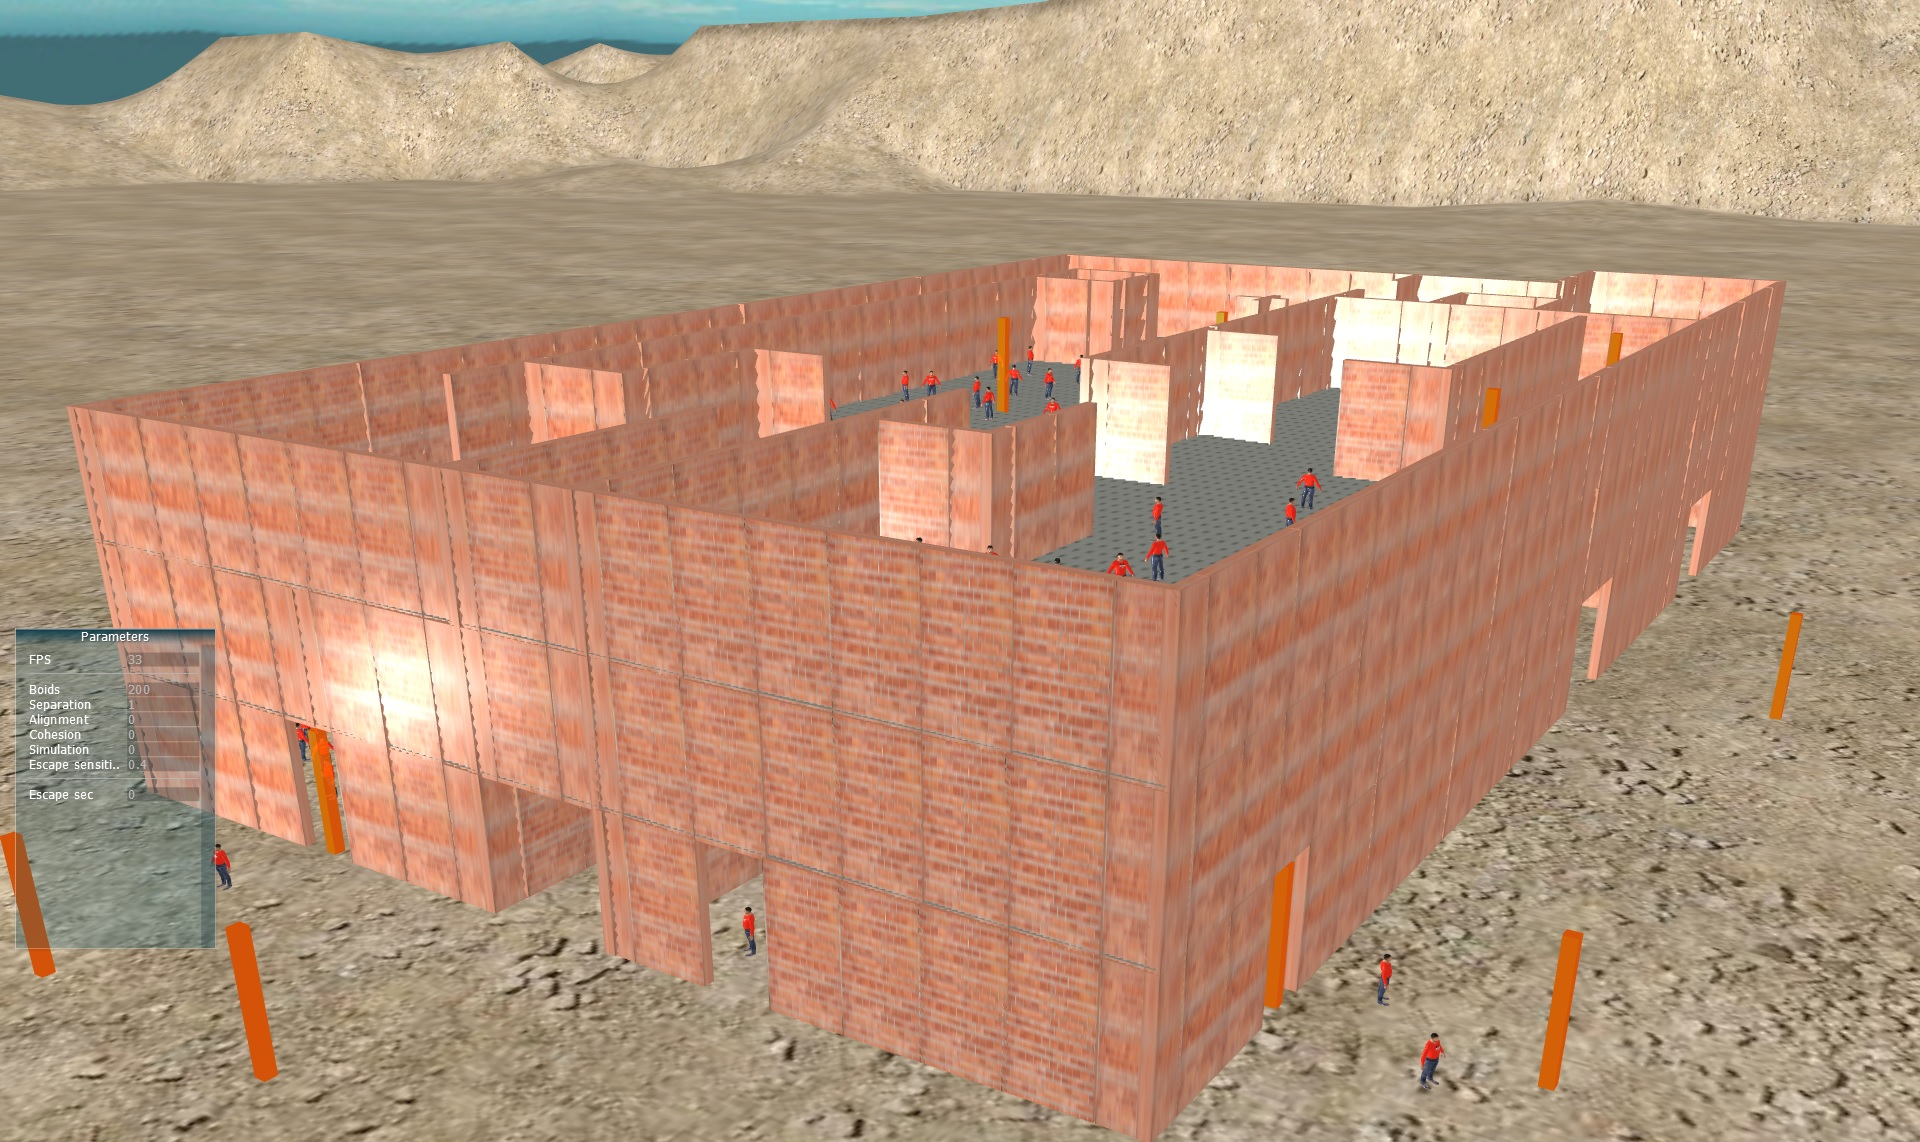
\includegraphics[width=0.9\textwidth]{Figures/screen8.jpg}
	\caption{Vyrenderovaná dvoupatrová budova}
\end{figure}

\begin{figure}[H]\centering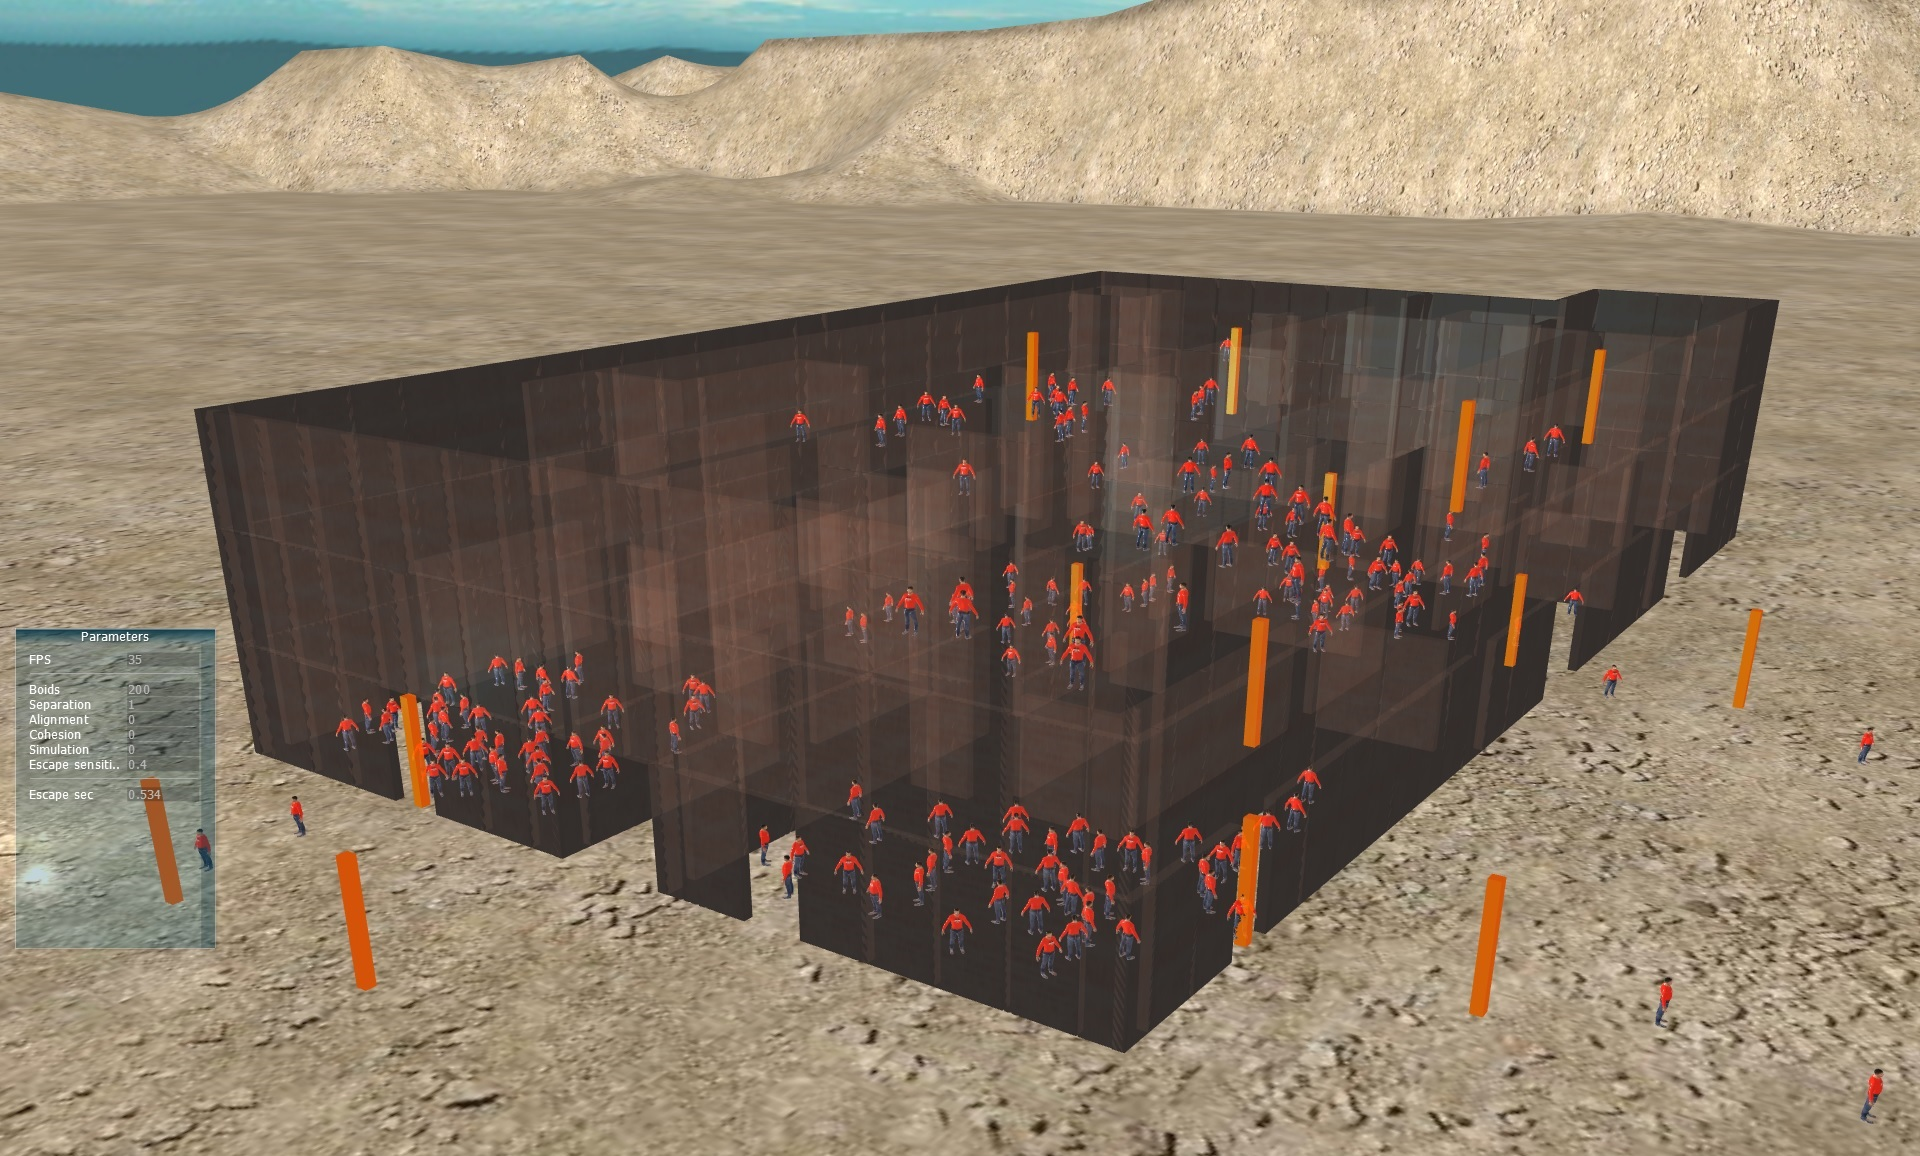
\includegraphics[width=0.9\textwidth]{Figures/screen6.jpg}
	\caption{Budova přepnuta do průhledného režimu se zviditelněním agentů a únikových bodů}
\end{figure}

\begin{figure}[H]\centering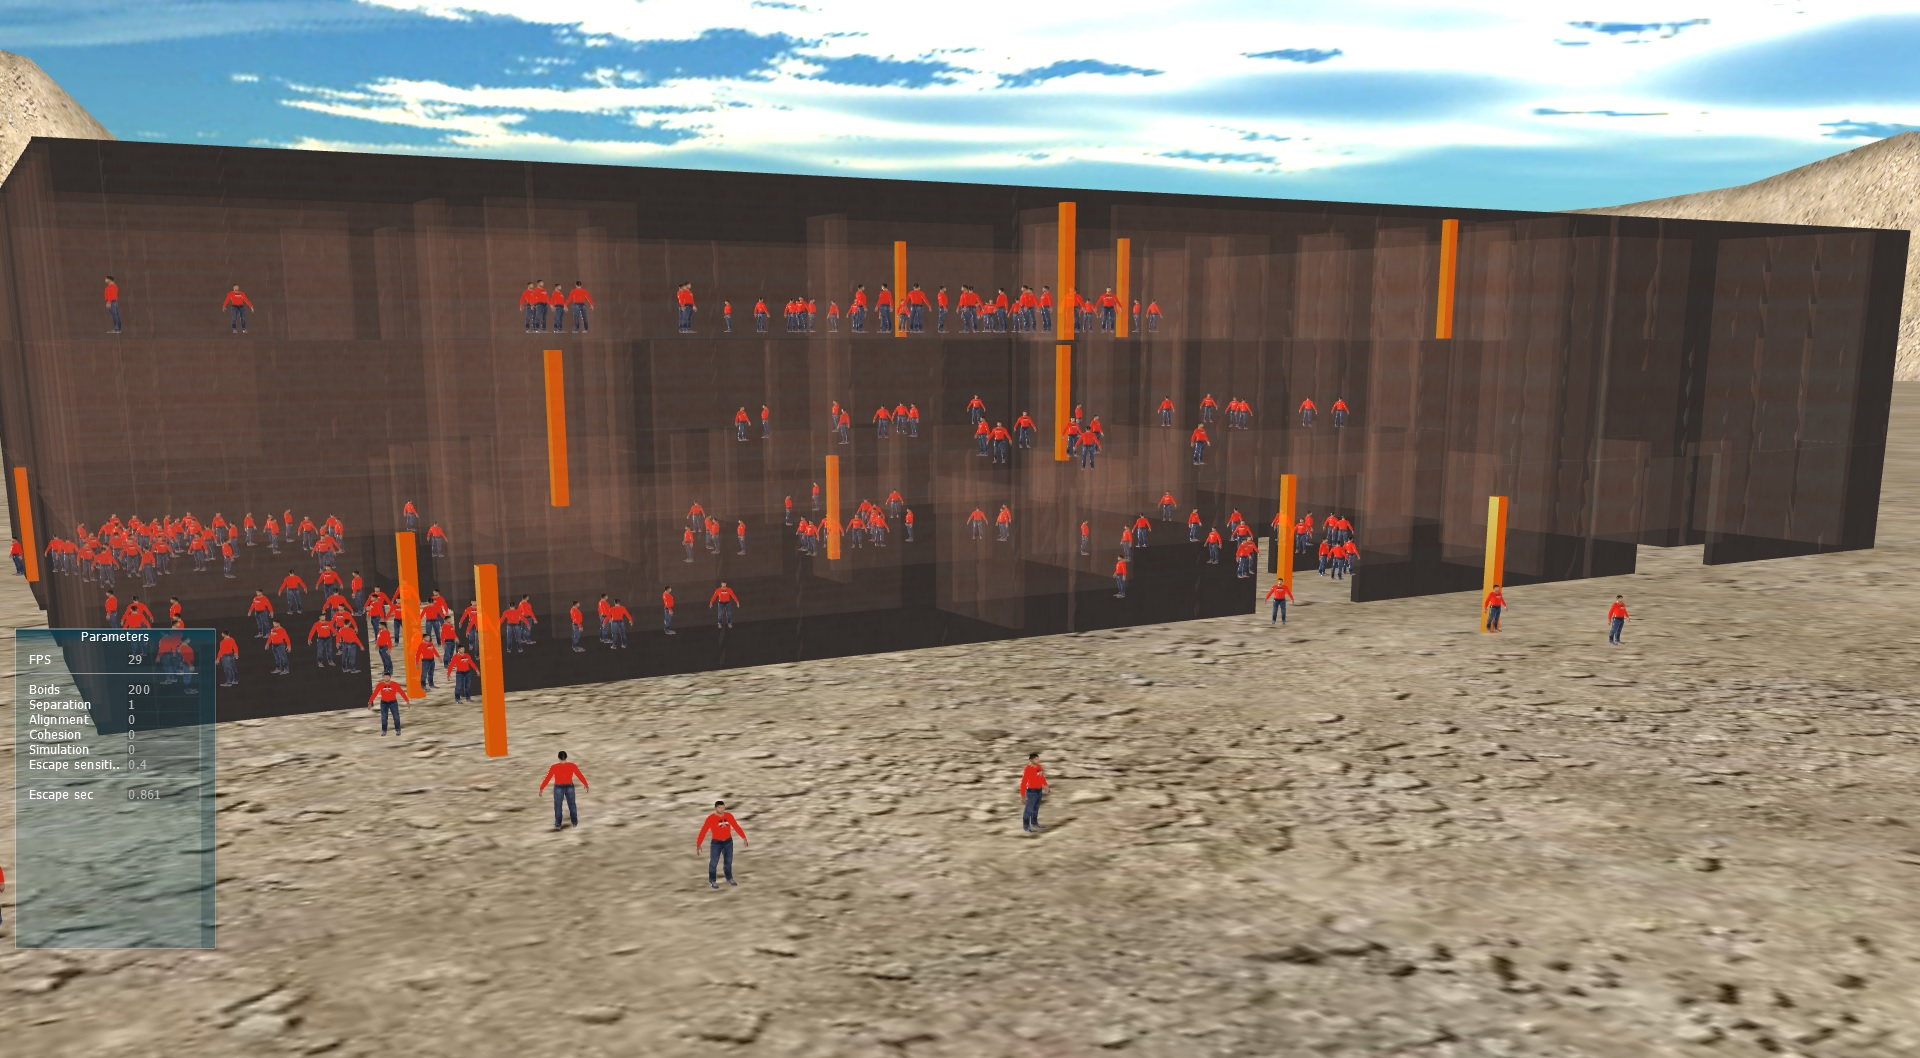
\includegraphics[width=0.9\textwidth]{Figures/screen7.jpg}
	\caption{Průhledný režim budovy z boční perspektivy}
\end{figure}

\begin{figure}[H]\centering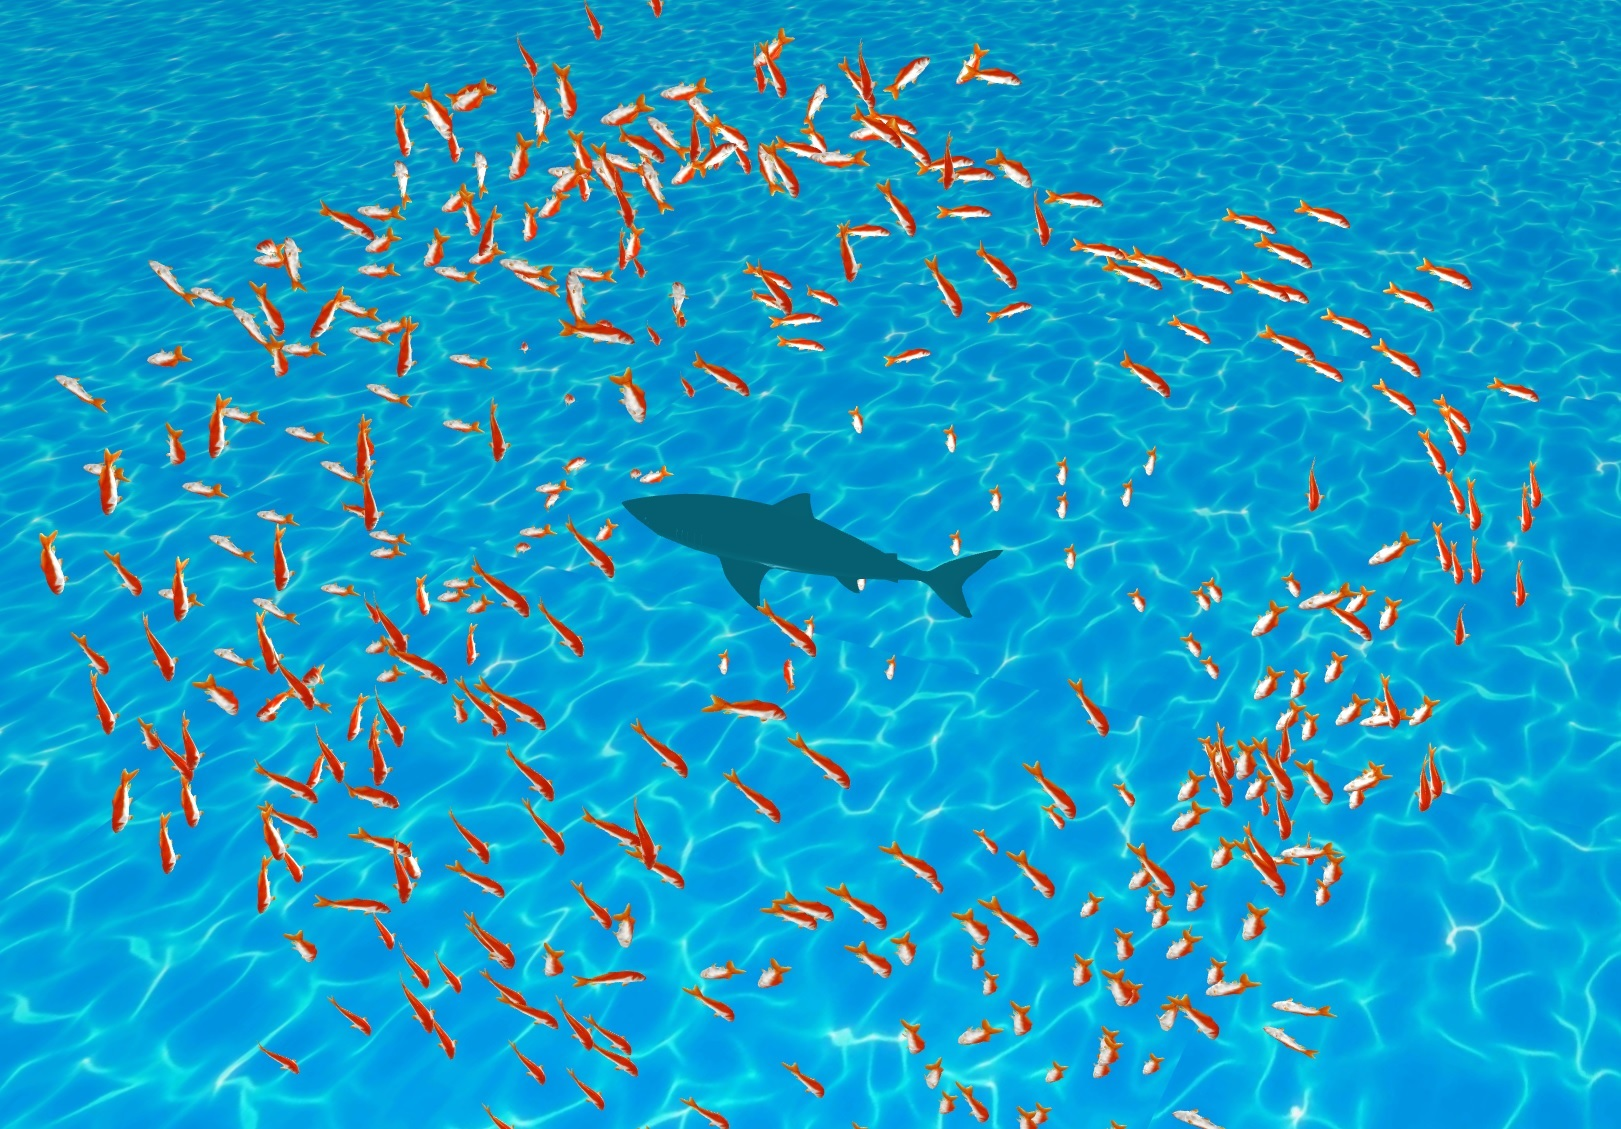
\includegraphics[width=0.9\textwidth]{Figures/new_fish4.jpg}\label{fig:hejnoRyb}
	\caption{Vyrenderované hejno ryb s vyhnutím se objektu}\label{fig:hejnoRyb}
\end{figure}

\section{Závěr}
Výsledkem této práce je aplikace, která má za úkol zrealizovat simulační algoritmus davu. Teoreticky byly popsány dvě varianty simulace (částicová simulace a simulace na bázi AI - umělé inteligence), z níž pro realizaci byla vybrána simulace na bázi AI a~pro implementaci byl vybrán Boidův algoritmus. V první možnosti využití v případě evakuace budovy se Boidův algoritmus a~jeho vylepšení neosvědčil na plno, avšak pro simulaci hejna byl vyhodnocen jako plně dostačující a využitelný v mnoha odvětví.

Aplikace nabízí dvě možnosti využití. První, jak již bylo zmíněno, je simulace úniku lidí z bodovy a druhá je využití obecného Boidova algoritmu jakožto simulace hejna (v této práci hejno ryb). U první varianty je možnost nadefinovat si vlastní schéma budovy včetně únikových východů a~u~druhé je možnost nadefinovat počet objektů, jimiž se bude hejno vyhýbat a~typ kolizního objektu, ve kterém se hejno pohybuje, a sice sféra (sphere) nebo krychle (cube). Uživatel si tak může vyzkoušet na obou příkladech výhody a nevýhody Boidova algoritmu a~také vliv jednotlivých parametrů na výslednou scénu.

\newpage

\begin{thebibliography}{99}
	
	\bibitem{linkToBuildingSimulation} Oasys,
	\textit{Crowd Simulation}, [online]. 2018 [cit. 2018-2-1]\\
	Dostupné z: \href{http://www.oasys-software.com/products/engineering/massmotion.html}{\texttt{http://www.oasys-software.com/products/engineering/massmotion.html}}
	
	\bibitem{linkToArmySimulation} FAAC Military,
	, [online]. 2018 [cit. 2018-2-1]\\
	Dostupné z: \href{https://www.faac.com/military/}{\texttt{https://www.faac.com/military/}}
	
	\bibitem{link1} Journal of the royal society interface, 
		\textit{Crowd behaviour during high-stress evacuations in an immersive virtual environment}, [online]. 2016 [cit. 2018-2-1]\\
		Dostupné z: \href{http://rsif.royalsocietypublishing.org/content/13/122/20160414}{\texttt{http://rsif.royalsocietypublishing.org/content/13/122/20160414}}
	
	\bibitem{link2} Boids, 
		\textit{Background and Update by Craig Reynolds}, [online]. 2018 [cit. 2018-2-1]\\
		Dostupné z: \href{https://www.red3d.com/cwr/boids/}{\texttt{https://www.red3d.com/cwr/boids/}}
	
	\bibitem{linkToUnrealEngineFish} Unreal Engine 4 \textit{simulace ryb}, [online]. 2016 [cit. 2018-2-1]\\
		Dostupné z: \href{		http://blog.csdn.net/nosix/article/details/52859160}{\texttt{		http://blog.csdn.net/nosix/article/details/52859160}}
	
	\bibitem{linkToCrytek} Crytek, [online]. 2018 [cit. 2018-4-19]\\
	Dostupné z: \href{http://www.crytek.com/}{\texttt{http://www.crytek.com/}}
	
	\bibitem{link3} The nature of code, 
		\textit{Chapter 6. Autonomous Agents}, [online]. 2018 [cit. 2018-2-1]\\
		Dostupné z: \href{http://natureofcode.com/book/chapter-6-autonomous-agents/}{\texttt{http://natureofcode.com/book/chapter-6-autonomous-agents/}}

	\bibitem{link4} Boids Pseudocode, 
		[online]. 2018 [cit. 2018-2-1]\\
		Dostupné z: \href{http://www.kfish.org/boids/pseudocode.html}{\texttt{http://www.kfish.org/boids/pseudocode.html}}
		
	\bibitem{linkToSimulation} Simulace,
		\textit{Glosář Aldebaran}, [online]. 2018 [cit. 2018-2-1]\\
		Dostupné z: \href{http://www.aldebaran.cz/glossary/print.php?id=1299}{\texttt{http://www.aldebaran.cz/glossary/print.php?id=1299}}
		
	
		
	\bibitem{linkToSimulationSpace} Earthlight,
		\textit{Spacewalk}, [online]. 2018 [cit. 2018-2-1]\\
		Dostupné z: \href{http://www.earthlightvr.com/spacewalk/}{\texttt{http://www.earthlightvr.com/spacewalk/}}
		
	\bibitem{linkToIteration} Techopedia,
		\textit{Iteration}, [online]. 2018 [cit. 2018-2-1]\\
		Dostupné z: \href{https://www.techopedia.com/definition/3821/iteration}{\texttt{https://www.techopedia.com/definition/3821/iteration}}
		
	\bibitem{linkToACM} ACM,
		\textit{Association for Computing Machinery}, [online]. 2018 [cit. 2018-2-1]\\
		Dostupné z: \href{https://www.acm.org/about-acm/what-is-acm}{\texttt{https://www.acm.org/about-acm/what-is-acm}}
		
	\bibitem{linkToSIGGRAPH} SIGGRAPH, [online]. 2018 [cit. 2018-2-1]\\
		Dostupné z: \href{https://www.siggraph.org/about/what-is-acm-siggraph}{\texttt{https://www.siggraph.org/about/what-is-acm-siggraph}}
		
	\bibitem{linkToBachelor1} Simulace davu, Mgr. Jan Stria,\\
		\textit{Matematicko-fyzikální fakulta (MFF)}, [online]. 2018 [cit. 2018-2-1]\\
		Dostupné z: \href{https://is.cuni.cz/webapps/zzp/detail/60388/}{\texttt{https://is.cuni.cz/webapps/zzp/detail/60388/}}
		
	\bibitem{linkToSteeringBehaviors} Steering Behaviors For Autonomous Characters\\
		\textit{Craig W. Reynolds}, [online]. 2018 [cit. 2018-2-1]\\
		Dostupné z: \href{http://www.red3d.com/cwr/steer/gdc99/}{\texttt{http://www.red3d.com/cwr/steer/gdc99/}}
		
	\bibitem{linkToCohesion} Kohezní síla,
		\textit{Glosář Aldebaran}, [online]. 2018 [cit. 2018-2-1]\\
		Dostupné z: \href{http://www.aldebaran.cz/glossary/print.php?id=1894}{\texttt{http://www.aldebaran.cz/glossary/print.php?id=1894}}
		
	\bibitem{linkToIDE} Techopedia,
		\textit{IDE}, [online]. 2018 [cit. 2018-2-4]\\
		Dostupné z:\\ \href{https://www.techopedia.com/definition/26860/integrated-development-environment-ide}{\texttt{https://www.techopedia.com/definition/26860/integrated-development-environment-ide}}
		
	\bibitem{linkToCppReference} CppReference.com,
		, [online]. 2018 [cit. 2018-2-4]\\
		Dostupné z: \href{http://en.cppreference.com/w/}{\texttt{http://en.cppreference.com/w/}}
		
	\bibitem{linkToPreIncrementation} CppReference.com,
		\textit{Increment/decrement operators}, [online]. 2018 [cit. 2018-2-4]\\
		Dostupné z: \href{http://en.cppreference.com/w/cpp/language/operator\_incdec}{\texttt{http://en.cppreference.com/w/cpp/language/operator\_incdec}}
		
	\bibitem{linkToTopIDE} Top IDE Index,
		[online]. 2018 [cit. 2018-2-4]\\
		Dostupné z: \href{https://pypl.github.io/IDE.html}{\texttt{https://pypl.github.io/IDE.html}}
		
	\bibitem{linkToVisualStudio} Visual Studio IDE,
		[online]. 2018 [cit. 2018-2-4]\\
		Dostupné z: \href{https://www.visualstudio.com}{\texttt{https://www.visualstudio.com}}
		
	\bibitem{linkToOpenGL} OpenGL,
		[online]. 2018 [cit. 2018-2-4]\\
		Dostupné z: \href{https://www.opengl.org/}{\texttt{https://www.opengl.org/}}
		
	\bibitem{linkToGLFW} GLFW,
		[online]. 2018 [cit. 2018-2-4]\\
		Dostupné z: \href{http://www.glfw.org/}{\texttt{http://www.glfw.org/}}
		
	\bibitem{linkToGLew} GLEW,
		[online]. 2018 [cit. 2018-2-4]\\
		Dostupné z: \href{http://glew.sourceforge.net/}{\texttt{http://glew.sourceforge.net//}}
		
	\bibitem{linkToGLM} GLM,
		[online]. 2018 [cit. 2018-2-4]\\
		Dostupné z: \href{https://glm.g-truc.net/0.9.8/index.html}{\texttt{https://glm.g-truc.net/0.9.8/index.html}}
		
	\bibitem{linkToAssimp} Assimp,
		[online]. 2018 [cit. 2018-2-4]\\
		Dostupné z: \href{http://assimp.sourceforge.net/}{\texttt{http://assimp.sourceforge.net/}}
		
	\bibitem{linkToStb} Stb image,
		[online]. 2018 [cit. 2018-2-4]\\
		Dostupné z: \href{https://github.com/nothings/stb}{\texttt{https://github.com/nothings/stb}}
		
	\bibitem{linkToOpenCV} OpenCV,
		[online]. 2018 [cit. 2018-2-4]\\
		Dostupné z: \href{https://opencv.org/}{\texttt{https://opencv.org/}}
		
	\bibitem{linkToAntTweakBar} AntTweakBar,
		[online]. 2018 [cit. 2018-2-13]\\
		Dostupné z: \href{http://anttweakbar.sourceforge.net/doc/}{\texttt{http://anttweakbar.sourceforge.net/doc/}}
		
\end{thebibliography}


\appendix
\section*{Přílohy}

Součástí přiloženého CD je:

\begin{itemize}
	\item Elektronická verze této práce ve formátu PDF.
	\item Zdrojové kódy demonstrační aplikace.
	\item Spustitelný soubor demonstrační aplikace.
\end{itemize}

\end{document}
